\documentclass[12pt,a4paper]{article}
\usepackage[a4paper, margin=0.8in, headheight=14pt]{geometry}
\usepackage{fontspec}
\usepackage{unicode-math}
\setmainfont{TeX Gyre Pagella}
\setmonofont[Scale=0.88]{TeX Gyre Cursor}
\setmathfont{Latin Modern Math}
\usepackage{xcolor}
\usepackage{colortbl}
\usepackage{titlesec}
\usepackage{enumitem}
\usepackage{tabularx}
\usepackage{booktabs}
\usepackage{array}
\usepackage{amsmath}
\usepackage{tikz}
\usetikzlibrary{shapes.geometric, arrows.meta, positioning, calc, fit, decorations.pathreplacing, decorations.pathmorphing}
\usepackage{tcolorbox}
\tcbuselibrary{skins, breakable}
\usepackage{hyperref}
\usepackage{fancyhdr}
\usepackage{graphicx}
\usepackage{microtype}
\hyphenpenalty=10000
\exhyphenpenalty=10000
\sloppy
\usepackage{caption}
\usepackage{setspace}
\usepackage{multirow}
\usepackage{tocloft}
\newcommand{\Q}[1]{\textbf{#1}\par\noindent\ignorespaces}
\definecolor{myred}{RGB}{196,30,58}
\definecolor{mydark}{RGB}{30,30,50}
\definecolor{mygreen}{RGB}{14,120,80}
\definecolor{myteal}{RGB}{0,130,140}
\definecolor{myamber}{RGB}{180,100,0}
\definecolor{mypurple}{RGB}{100,30,160}
\definecolor{mygray}{RGB}{246,247,249}
\definecolor{mgframe}{RGB}{180,185,200}
\definecolor{watermark}{RGB}{145,150,170}
\definecolor{hdrred}{RGB}{250,232,235}
\definecolor{hdrgreen}{RGB}{220,244,233}
\definecolor{hdrteal}{RGB}{220,242,244}
\definecolor{hdramber}{RGB}{253,242,215}
\definecolor{hdrpurple}{RGB}{238,228,255}
\definecolor{hdrgray}{RGB}{238,240,245}
\definecolor{rowalt}{RGB}{250,251,253}

\titleformat{\section}{\large\bfseries\color{myred}}{\thesection.}{0.5em}{}[\vspace{1pt}{\color{myred}\rule{\linewidth}{0.8pt}}]
\titleformat{\subsection}{\normalsize\bfseries\color{myteal}}{\thesubsection}{0.5em}{}
\titlespacing*{\section}{0pt}{18pt}{7pt}
\titlespacing*{\subsection}{0pt}{11pt}{4pt}
\setlength{\parindent}{0pt}
\setlength{\parskip}{4pt}
\renewcommand{\cfttoctitlefont}{\large\bfseries\color{myred}}
\renewcommand{\cftaftertoctitle}{\par\noindent{\color{myred}\rule{\linewidth}{0.8pt}}}
\setlength{\cftbeforetoctitleskip}{0pt}
\setlength{\cftaftertoctitleskip}{6pt}
\renewcommand{\cftsecfont}{\normalsize\bfseries\color{mydark}}
\renewcommand{\cftsecpagefont}{\normalsize\bfseries\color{mydark}}
\renewcommand{\cftsecleader}{\cftdotfill{\cftdotsep}}
\setlength{\cftbeforesecskip}{7pt}
\renewcommand{\cftsubsecfont}{\small\color{mydark}}
\renewcommand{\cftsubsecpagefont}{\small\color{mydark}}
\setlength{\cftbeforesubsecskip}{3pt}
\setlength{\cftsubsecindent}{1.4em}
\renewcommand{\cftpartfont}{\normalsize\bfseries\color{myteal}}
\renewcommand{\cftpartpagefont}{\normalsize\bfseries\color{myteal}}
\setlength{\cftbeforepartskip}{14pt}
\renewcommand{\arraystretch}{1.45}
\setlength{\tabcolsep}{6pt}
\arrayrulecolor{mydark}
\newcolumntype{B}[1]{>{\small\bfseries\raggedright\arraybackslash}m{#1}}
\newcolumntype{C}[1]{>{\centering\arraybackslash}m{#1}}
\newcolumntype{Y}{>{\small\raggedright\arraybackslash}X}
\renewcommand{\tabularxcolumn}[1]{m{#1}}
\newcommand{\currmodule}{Module 1}
\pagestyle{fancy}
\fancyhf{}
\fancyhead[L]{\small\color{myred}\textbf{PE-EC701C}\;\color{mydark}--- Mobile Communication and Networks}
\fancyhead[R]{\small\color{myteal}\textbf{\currmodule\ Notes}}
\fancyfoot[C]{\small\color{mydark}\thepage}
\fancyfoot[R]{\small\color{watermark}\textit{\copyright\ Biraj}}
\renewcommand{\headrulewidth}{0.5pt}
\renewcommand{\footrulewidth}{0.3pt}

\hypersetup{colorlinks=true, linkcolor=myteal, urlcolor=myteal,
  pdfauthor={Biraj Sarkar},
  pdftitle={PE-EC701C --- Combined Notes}}

\tcbset{
  tikzbox/.style={
    colback=mygray, colframe=mgframe, boxrule=0.6pt, arc=4pt,
    left=8pt, right=8pt, top=6pt, bottom=6pt,
    colbacktitle=mgframe, coltitle=mydark,
    fonttitle=\small\bfseries
  },
  defbox/.style={
    colback=hdrgreen, colframe=mygreen, boxrule=0.8pt, arc=4pt,
    left=9pt, right=9pt, top=6pt, bottom=6pt,
    colbacktitle=mygreen, coltitle=white,
    fonttitle=\small\bfseries
  },
  formulabox/.style={
    colback=hdrteal, colframe=myteal, boxrule=0.8pt, arc=4pt,
    left=9pt, right=9pt, top=7pt, bottom=7pt,
    colbacktitle=myteal, coltitle=white,
    fonttitle=\small\bfseries
  },
  examplebox/.style={
    colback=hdramber, colframe=myamber, boxrule=0.8pt, arc=4pt,
    left=9pt, right=9pt, top=6pt, bottom=6pt,
    colbacktitle=myamber, coltitle=white,
    fonttitle=\small\bfseries
  },
  masonbox/.style={
    colback=hdrpurple, colframe=mypurple, boxrule=0.8pt, arc=4pt,
    left=9pt, right=9pt, top=6pt, bottom=6pt,
    colbacktitle=mypurple, coltitle=white,
    fonttitle=\small\bfseries
  },
  exambox/.style={
    colback=hdrpurple, colframe=mypurple, boxrule=1pt, arc=5pt,
    left=10pt, right=10pt, top=8pt, bottom=8pt,
    colbacktitle=mypurple, coltitle=white,
    fonttitle=\bfseries,
    breakable, title after break={\textbf{Frequently Asked / Viva Questions (contd.)}}}
}
\tcbset{breakable}
\tcbset{after={\color{black}}}

\tikzset{
  block/.style={rectangle, draw=myteal, fill=hdrteal,
    text width=2.4cm, align=center, minimum height=0.95cm,
    font=\small, rounded corners=3pt, line width=0.7pt},
  redblock/.style={rectangle, draw=myred, fill=hdrred,
    text width=2.4cm, align=center, minimum height=0.95cm,
    font=\small, rounded corners=3pt, line width=0.7pt},
  netnode/.style={rectangle, draw=myteal, fill=hdrteal,
    text width=1.5cm, align=center, minimum height=0.8cm,
    font=\small, rounded corners=3pt, line width=0.7pt},
  sumjunc/.style={circle, draw=myamber, fill=hdramber,
    minimum size=0.62cm, font=\small, line width=0.8pt},
  snode/.style={circle, draw=mypurple, fill=hdrpurple,
    minimum size=0.55cm, font=\footnotesize, line width=0.7pt},
  arrow/.style={-Stealth, thick, color=mydark},
  redarrow/.style={-Stealth, thick, color=myred},
  line/.style={thick, color=mydark},
  hexagon/.style={
    regular polygon, regular polygon sides=6,
    draw=myteal, fill=hdrteal, minimum size=1.8cm, inner sep=0pt,
    line width=0.8pt, rotate=30
  }
}

\newcommand{\modulestart}[2]{%
  \clearpage
  \renewcommand{\currmodule}{Module #1}%
  \renewcommand{\theHsection}{mod#1.\arabic{section}}%
  \renewcommand{\theHsubsection}{\theHsection.\arabic{subsection}}%
  \renewcommand{\theHsubsubsection}{\theHsubsection.\arabic{subsubsection}}%
  \phantomsection
  \addcontentsline{toc}{part}{Module #1: #2}%
  \setcounter{section}{0}%
  \begin{center}
    \vspace*{1.0cm}
    {\Huge\bfseries\color{myred} Module #1}\\[10pt]
    {\Large\bfseries\color{mydark} #2}\\[10pt]
    {\color{myred}\rule{0.55\linewidth}{1.2pt}}
  \end{center}
  \vspace{14pt}
}
\begin{document}

\thispagestyle{empty}
\vspace*{1.0cm}
\begin{center}
  {\Huge\bfseries\color{myred} PE-EC701C}\\[10pt]
  {\LARGE\bfseries\color{mydark} Mobile Communication and Networks}\\[20pt]
  {\color{myred}\rule{0.7\linewidth}{1.5pt}}\\[18pt]
  {\Large\color{myteal}\textbf{Combined Module Notes}}\\[8pt]
  {\large\color{mydark} Modules 1 -- 6}\\[40pt]
  {\normalsize\color{mydark} Semester VII \quad$\bullet$\quad 3L:0T:0P \quad$\bullet$\quad 3 Credits}\\[12pt]
  {\normalsize\color{mydark} CGEC \;$|$\; B.Tech ECE (2023--27)}\\[6pt]
  {\normalsize\color{mydark}\textit{Biraj Sarkar}}
\end{center}
\vspace{1.0cm}
\begin{center}
  \begin{tcolorbox}[colback=mygray, colframe=mgframe, boxrule=0.5pt, arc=3pt, width=0.85\linewidth]
    \centering\small\color{mydark}
    \textbf{Disclaimer / Study Guide Notice:}\\
    These are condensed \textbf{Short Notes} focusing on core theory, key formulas, block/circuit diagrams, and standard viva Q\&As for university exam revision. Exhaustive numerical practice problems and derivation edge cases are not covered. This serves as a quick-revision reference guide for students.
  \end{tcolorbox}
\end{center}
\vfill
\begin{center}{\small\color{watermark}\textit{Exam-Ready Notes}}\end{center}
\clearpage

\hypersetup{linkcolor=mydark}
\tableofcontents
\hypersetup{linkcolor=myteal}
\clearpage

% -- Module 1 -----------------------------------------------------------------
\modulestart{1}{Cellular Concepts and Cell Structure}

\section{Cellular Concepts and Cell Structure}
% ===============================================================================

Early mobile radio systems utilized high-power transmitters on tall towers to achieve maximum coverage. This centralized approach suffered from severe spectral congestion and could support only a handful of simultaneous users. The cellular concept solved this by replacing a single large transmitter with many low-power transmitters distributed across the service area.

\begin{tcolorbox}[defbox]
\textbf{Cellular System:} A system in which a geographical area is partitioned into smaller, adjacent subdivisions called \textbf{cells}, each served by its own low-power base station (BS). By limiting transmitter range, the same frequency channels can be reused by different cells at a safe distance, dramatically increasing network capacity.
\end{tcolorbox}

\subsection{Hexagonal Cell Geometry}
Although real-world cell coverage areas are irregular (due to terrain, buildings, and signal propagation), simplified geometric models are used for system design:
\begin{itemize}[leftmargin=*, itemsep=3pt]
  \item \textbf{Circle:} Represents ideal radiation patterns but cannot be tiled. In overlapping circular configurations, gaps or double-coverage zones occur.
  \item \textbf{Square / Triangle:} Can tile an area without gaps, but the distance from the cell center to its boundary varies heavily, leading to poor cell-edge performance.
  \item \textbf{Hexagon:} The ideal choice. It tiles the plane without gaps or overlaps, closely approximates a circle (ideal omnidirectional radiation), and has the largest area for a given distance to its corners, minimizing the number of cells required to cover a region.
\end{itemize}

% ===============================================================================
\section{Frequency Reuse and Capacity}
% ===============================================================================

Frequency reuse is the core mechanism of cellular systems. It allows a fixed allocation of RF spectrum to support an arbitrary number of users.

\begin{tcolorbox}[defbox]
\textbf{Frequency Reuse:} The design technique of dividing the total available channels into smaller, distinct groups and assigning these groups to different cells, such that cells operating on the same frequency group are physically separated by a distance large enough to keep interference below a tolerable limit.
\end{tcolorbox}

\subsection{Cluster and Geometry Formulation}
Let the total number of duplex channels allocated to the system be $S$. These channels are divided into $N$ orthogonal channel groups, each group containing $k$ channels ($S = k N$).
\begin{itemize}[leftmargin=*, itemsep=2.5pt]
  \item \textbf{Cluster Size ($N$):} The group of $N$ cells that collectively use the entire set of available frequencies. No two cells in a single cluster can share frequencies.
  \item Because of hexagonal geometry constraints, $N$ can only take values that satisfy:
    \begin{equation}
      N = i^2 + ij + j^2 \quad \text{where } i, j \in \{0, 1, 2, \dots\}
    \end{equation}
    Typical values are $N = 1, 3, 4, 7, 9, 12, 19, 21, \dots$
  \item \textbf{System Capacity ($C$):} If a cluster of size $N$ is replicated $M$ times across the system:
    \begin{equation}
      C = M \cdot S = M \cdot k \cdot N
    \end{equation}
\end{itemize}

\subsection{Co-channel Reuse Ratio}
Cells that use the same channel group are called \textbf{co-channel cells}. Let $R$ be the cell radius (distance from center to vertex) and $D$ be the minimum distance between co-channel cell centers.
\begin{tcolorbox}[formulabox, title={\textbf{Co-channel Reuse Distance and Ratio}}]
For a hexagonal grid, the co-channel reuse distance $D$ is given by:
\begin{equation}
  D = R \sqrt{3N}
\end{equation}
The co-channel reuse ratio $Q$ represents the spatial separation normalized by the cell radius:
\begin{equation}
  Q = \frac{D}{R} = \sqrt{3N}
\end{equation}
\textbf{Significance:} A small value of $Q$ implies small cluster size $N$, allowing high frequency reuse and high capacity, but results in higher co-channel interference. A large value of $Q$ reduces interference but lowers capacity.
\end{tcolorbox}

\begin{tcolorbox}[tikzbox, title={7-Cell Frequency Reuse Cluster Pattern (N = 7)}]
\centering
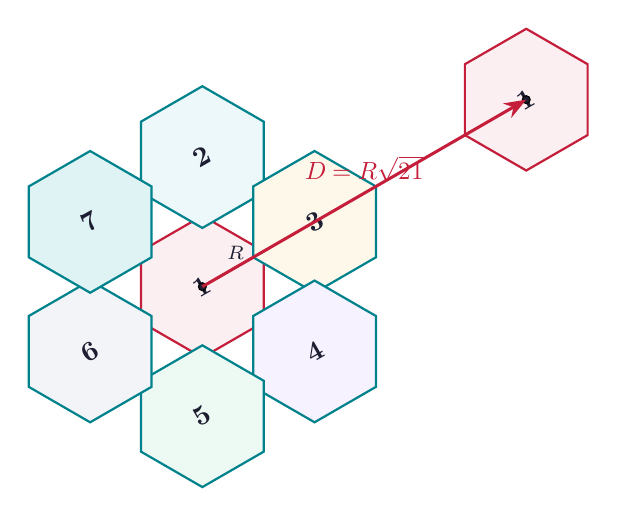
\begin{tikzpicture}[scale=0.95]
  % Define coordinates for 7-cell cluster
  % Centers at distance sqrt(3)*R = 1.732
  \node[hexagon, fill=hdrred!70, draw=myred] (c1) at (0,0) {\textbf{\color{mydark}1}};
  \node[hexagon, fill=hdrteal!50] (c2) at (0, 1.732) {\textbf{\color{mydark}2}};
  \node[hexagon, fill=hdramber!50] (c3) at (1.5, 0.866) {\textbf{\color{mydark}3}};
  \node[hexagon, fill=hdrpurple!50] (c4) at (1.5, -0.866) {\textbf{\color{mydark}4}};
  \node[hexagon, fill=hdrgreen!50] (c5) at (0, -1.732) {\textbf{\color{mydark}5}};
  \node[hexagon, fill=hdrgray!70] (c6) at (-1.5, -0.866) {\textbf{\color{mydark}6}};
  \node[hexagon, fill=hdrteal!90] (c7) at (-1.5, 0.866) {\textbf{\color{mydark}7}};

  % Label showing radius R
  \draw[line, dashed] (0,0) -- (0.9, 0.519) node[midway, above=-1pt, font=\scriptsize] {$R$};
  \draw[fill=mydark] (0,0) circle (1.5pt);

  % Draw a second co-channel cell '1' to show reuse distance D
  % Shift center by i=2, j=1 steps -> distance for N=7 is D = R*sqrt(21) = 4.58R approx 4.0cm
  % Shift: x = R*sqrt(3)*(i + j*cos(60)) = 1.732 * (2 + 0.5) = 4.33, y = R*sqrt(3)*j*sin(60) = 1.732 * 0.866 = 1.5
  \node[hexagon, fill=hdrred!70, draw=myred] (c1_reuse) at (4.33, 2.5) {\textbf{\color{mydark}1}};
  \draw[fill=mydark] (4.33, 2.5) circle (1.5pt);

  % Connect centers with arrow showing D
  \draw[arrow, redarrow, line width=1.1pt] (0,0) -- (4.33, 2.5) node[midway, above, font=\small\bfseries] {$D = R\sqrt{21}$};
\end{tikzpicture}
\end{tcolorbox}

% ===============================================================================
\section{Cell Splitting, Sectoring, and Microcell Zone Concept}
% ===============================================================================

When traffic demand in a cellular network exceeds the capacity of the allocated channels, the network must be densified or modified to support more users. Three primary strategies are used:

\subsection{Cell Splitting}
Cell splitting partitions congested cells into smaller cells (microcells), each with its own base station and a corresponding reduction in transmitter power.
\begin{itemize}[leftmargin=*, itemsep=3pt]
  \item \textbf{Mechanism:} By reducing the cell radius from $R$ to $R/2$, the area of the cell is reduced by a factor of 4. Since each microcell uses the same cluster design, the capacity per unit area increases by a factor of 4.
  \item \textbf{Power Scaling:} To maintain the same co-channel reuse ratio $Q$, the transmit power of the new microcell base stations must be reduced. Power scales as:
    \begin{equation}
      P_{\text{new}} = P_{\text{old}} \cdot \left(\frac{R_{\text{new}}}{R_{\text{old}}}\right)^n = \frac{P_{\text{old}}}{16} \quad (\text{for path loss exponent } n=4)
    \end{equation}
\end{itemize}

\begin{tcolorbox}[tikzbox, title={Cell Splitting Concept (Radius R divided by 2)}]
\centering
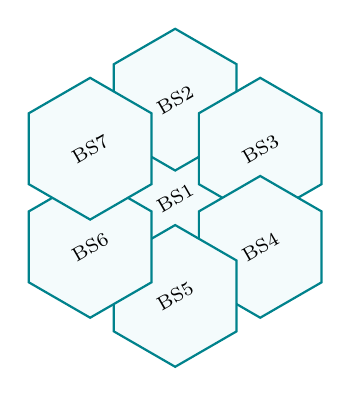
\begin{tikzpicture}[scale=0.8]
  % Original large hexagon
  \node[hexagon, minimum size=3.6cm, fill=none, draw=mydark, dashed, line width=1pt] (h1) at (0,0) {};
  \node at (0, 1.3) {\small Original Cell ($R$)};
  
  % Split hexagons inside
  \node[hexagon, minimum size=1.8cm, fill=hdrteal!30] (s1) at (0,0) {\scriptsize BS1};
  \node[hexagon, minimum size=1.8cm, fill=hdrteal!30] (s2) at (0, 1.558) {\scriptsize BS2};
  \node[hexagon, minimum size=1.8cm, fill=hdrteal!30] (s3) at (1.35, 0.779) {\scriptsize BS3};
  \node[hexagon, minimum size=1.8cm, fill=hdrteal!30] (s4) at (1.35, -0.779) {\scriptsize BS4};
  \node[hexagon, minimum size=1.8cm, fill=hdrteal!30] (s5) at (0, -1.558) {\scriptsize BS5};
  \node[hexagon, minimum size=1.8cm, fill=hdrteal!30] (s6) at (-1.35, -0.779) {\scriptsize BS6};
  \node[hexagon, minimum size=1.8cm, fill=hdrteal!30] (s7) at (-1.35, 0.779) {\scriptsize BS7};
\end{tikzpicture}
\end{tcolorbox}

\subsection{Sectoring}
Instead of omnidirectional antennas, sectoring uses directional antennas at the base station to transmit only in specific directions.
\begin{itemize}[leftmargin=*, itemsep=3.5pt]
  \item \textbf{Principle:} Common configurations are $120^\circ$ sectoring (3 sectors per cell) and $60^\circ$ sectoring (6 sectors per cell).
  \item \textbf{Impact:} By directing transmission, a sector receives interference only from co-channel cells located within its antenna's main beam. This dramatically reduces the number of co-channel interferers, improving the Carrier-to-Interference ratio ($C/I$).
  \item \textbf{Trade-off:} Sectoring divides the channels of a cell into smaller groups, which reduces trunking efficiency and increases handoff frequency.
\end{itemize}

\subsection{Microcell Zone Concept}
To address the trunking efficiency loss and frequent handoffs of sectoring, the microcell zone concept is used.
\begin{itemize}[leftmargin=*, itemsep=3.5pt]
  \item A large cell is divided into three zone transmitters (microcells) located at the periphery, all connected to a single central base station via fiber or microwave link.
  \item As a mobile user moves within the cell, the base station dynamically switches the active zone transmitter. No handoff is triggered at the Mobile Switching Center (MSC) since all zones share the same channels and base station.
\end{itemize}

% ===============================================================================
\section{Channel Assignment and Handoff Strategies}
% ===============================================================================

\subsection{Channel Assignment Strategies}
To optimize spectrum utilization, channels are managed using one of two strategies:
\par\noindent
{\renewcommand{\arraystretch}{1.55}%
\begin{tabularx}{\linewidth}{|B{3.2cm}|Y|Y|}\hline
\textbf{Parameter} & \textbf{Fixed Channel Assignment (FCA)} & \textbf{Dynamic Channel Assignment (DCA)} \\[4pt]
\hline
\textbf{Allocation} & Channels are permanently assigned to each cell according to a reuse plan. & Channels are kept in a central pool and assigned on-demand. \\[4pt]
\hline
\textbf{Traffic Adaptability} & Poor. If a cell runs out of channels, calls are blocked, even if adjacent cells are idle. & Excellent. Adapts to real-time spatial traffic variations. \\[4pt]
\hline
\textbf{Complexity} & Very low. No real-time optimization or coordination required. & High. Requires real-time measurements and central control. \\[4pt]
\hline
\textbf{Interference Control} & Hardcoded safety distance protects against co-channel interference. & Requires continuous monitoring of signal levels to avoid collisions. \\[4pt]
\hline
\end{tabularx}
}

\subsection{Handoff Strategies}
\begin{tcolorbox}[defbox]
\textbf{Handoff (or Handover):} The process of transferring an active call or data session from one channel or base station to another as the mobile station moves between coverage areas.
\end{tcolorbox}

\begin{enumerate}[label=\textbf{\arabic*.}, leftmargin=*, itemsep=4pt]
  \item \textbf{Hard Handoff ("Break-before-make"):} The mobile station disconnects from the current base station before connecting to the target base station. Used in FDMA and TDMA systems. It is simple but can lead to dropped calls if the connection fails.
  \item \textbf{Soft Handoff ("Make-before-break"):} The mobile station connects to the new base station while maintaining its link with the current base station. Used in CDMA (spread-spectrum) systems. It ensures zero connection gap but consumes double channel resources during the handoff transition.
  \item \textbf{Delayed (or Two-Threshold) Handoff:} Employs a primary signal threshold to initiate handoff, but delays execution until a second, lower threshold is reached. Prevents unnecessary handoffs due to temporary signal fading.
  \item \textbf{Queuing Handoff:} Instead of blocking a handoff request if no channels are available in the target cell, the request is placed in a queue. Since handoff calls have higher priority than new calls, they are served as soon as a channel frees up.
\end{enumerate}

\begin{tcolorbox}[tikzbox, title={Handoff Thresholds and Hysteresis}]
\centering
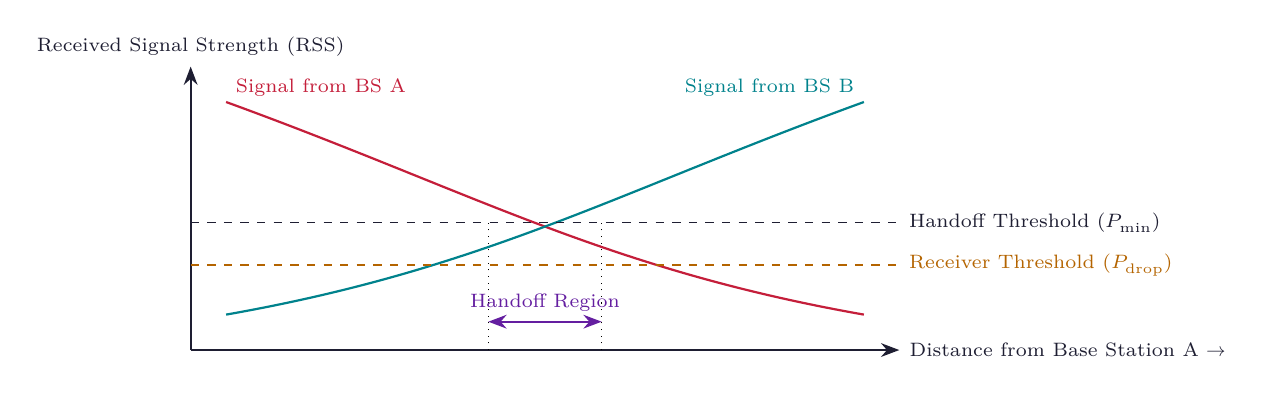
\begin{tikzpicture}[scale=0.9, every node/.style={font=\scriptsize}]
  % Axes
  \draw[arrow] (0,0) -- (10,0) node[right] {Distance from Base Station A $\to$};
  \draw[arrow] (0,0) -- (0,4) node[above] {Received Signal Strength (RSS)};

  % Curves representing signal strength from BS A and BS B
  \draw[thick, color=myred] (0.5, 3.5) to[out=-20, in=170] (9.5, 0.5);
  \node[color=myred, right] at (0.5,3.7) {Signal from BS A};
  
  \draw[thick, color=myteal] (0.5, 0.5) to[out=10, in=-160] (9.5, 3.5);
  \node[color=myteal, left] at (9.5,3.7) {Signal from BS B};

  % Threshold lines
  \draw[dashed, color=mydark] (0, 1.8) -- (10, 1.8) node[right] {Handoff Threshold ($P_{\text{min}}$)};
  \draw[dashed, color=myamber] (0, 1.2) -- (10, 1.2) node[right] {Receiver Threshold ($P_{\text{drop}}$)};

  % Vertical lines for intersections
  \draw[dotted] (4.2, 0) -- (4.2, 1.8);
  \draw[dotted] (5.8, 0) -- (5.8, 1.8);
  
  \draw[thick, Stealth-Stealth, color=mypurple] (4.2, 0.4) -- (5.8, 0.4) node[midway, above] {Handoff Region};
\end{tikzpicture}
\end{tcolorbox}

% ===============================================================================
\section{Interference, Capacity, and Power Control}
% ===============================================================================

\subsection{Co-channel Interference (CCI)}
CCI arises from cells using the same frequency channels. The Carrier-to-Interference ratio ($C/I$) determines signal quality:
\begin{equation}
  \frac{C}{I} = \frac{S}{\sum_{i=1}^{i_0} I_i}
\end{equation}
Where $S$ is the desired signal power and $I_i$ is the interference power from the $i$-th co-channel cell, and $i_0$ is the number of co-channel interferers (first tier).
Assuming propagation path loss follows a power law ($P_r \propto d^{-n}$):
\begin{equation}
  \frac{C}{I} = \frac{R^{-n}}{\sum_{i=1}^{i_0} D_i^{-n}} \approx \frac{(D/R)^n}{i_0} = \frac{(\sqrt{3N})^n}{i_0}
\end{equation}
Where $n$ is the path loss exponent. For a typical first-tier of 6 co-channel interferers ($i_0 = 6$):
\begin{equation}
  \frac{C}{I} \approx \frac{(3N)^{n/2}}{6}
\end{equation}

\subsection{Adjacent Channel Interference (ACI)}
ACI is caused by signals in adjacent frequency bands. It occurs due to imperfect receiver filtering, which allows nearby frequencies to leak into the passband (spectral regrowth).
\begin{itemize}[leftmargin=*, itemsep=2.5pt]
  \item \textbf{Mitigation:} Guard bands are inserted between channel allocations, and adjacent channels are never assigned to the same cell or adjacent cells in the reuse pattern.
\end{itemize}

\subsection{Trunking and Capacity Measures (Erlang)}
Trunking exploits the statistical behavior of users, allowing a small number of channels to serve a much larger user base.
\begin{itemize}[leftmargin=*, itemsep=3pt]
  \item \textbf{Traffic Intensity ($A$):} Measured in \textbf{Erlangs} (dimensionless unit of traffic). For $U$ users, each with call request rate $\lambda$ and average call duration $H$:
    \begin{equation}
      A = U \cdot A_u = U \cdot (\lambda H)
    \end{equation}
  \item \textbf{Erlang B (Blocked Calls Cleared):} Determines the probability of a call being blocked ($P_b$) when no channels are available. Calls are cleared immediately.
    \begin{equation}
      P_b = \frac{\frac{A^C}{C!}}{\sum_{k=0}^{C} \frac{A^k}{k!}} \quad (C = \text{number of channels})
    \end{equation}
  \item \textbf{Erlang C (Blocked Calls Delayed):} Assumes blocked calls enter a queue, calculating the probability of a call experiencing a delay.
\end{itemize}

\subsection{Power Control}
Power control dynamically adjusts the transmitter power of mobile units and base stations.
\begin{itemize}[leftmargin=*, itemsep=3pt]
  \item \textbf{Need:} Solves the \textbf{Near-Far Problem} in CDMA, where a transmitter near the base station overrides weaker signals from distant users.
  \item \textbf{Open-Loop Power Control:} The mobile station estimates path loss based on the received pilot signal and adjusts its transmit power accordingly. It is fast but does not account for independent uplink fading.
  \item \textbf{Closed-Loop Power Control:} The base station measures the received signal SNR from the mobile station and sends power adjustment commands (up/down bits) via the downlink control channel. Highly accurate.
\end{itemize}

\newpage
% ===============================================================================
\section{Wireless Cellular Standards: 2G and 3G}
% ===============================================================================

Cellular networks transitioned from analog voice (1G) to digital systems (2G) and high-speed data networks (3G):

\par\noindent
{\renewcommand{\arraystretch}{1.55}%
\begin{tabularx}{\linewidth}{|B{3.2cm}|Y|Y|}\hline
\textbf{Feature} & \textbf{2G Cellular Standards} & \textbf{3G Cellular Standards} \\
\hline
\textbf{Primary Standards} & \textbf{GSM} (Global System for Mobile) and \textbf{IS-95} (cdmaOne). & \textbf{WCDMA} (UMTS) and \textbf{CDMA2000}. \\[4pt]
\hline
\textbf{Access Scheme} & TDMA/FDMA (GSM), CDMA (IS-95). & WCDMA (DS-CDMA), CDMA2000. \\
\hline
\textbf{Channel Bandwidth} & 200 kHz (GSM), 1.25 MHz (IS-95). & 5 MHz (WCDMA), 1.25 MHz (CDMA2000). \\[4pt]
\hline
\textbf{Data Rate} & 9.6 kbps (GSM), up to 144 kbps (IS-95B). & 384 kbps (UMTS) up to 2 Mbps (HSPA). \\[4pt]
\hline
\textbf{Voice/Data Type} & Digital voice, SMS, basic packet data (GPRS). & High-speed packet data, video calling, mobile internet. \\[4pt]
\hline
\textbf{Modulation} & GMSK (GSM), BPSK/QPSK (IS-95). & QPSK/16-QAM. \\
\hline
\end{tabularx}
}

\subsection{Evolutionary Paths}
\begin{itemize}[leftmargin=*, itemsep=3pt]
  \item \textbf{GSM to 3G:} GSM (9.6 kbps) $\to$ GPRS (General Packet Radio Service, 115 kbps) $\to$ EDGE (Enhanced Data Rates for GSM Evolution, 384 kbps, uses 8-PSK) $\to$ WCDMA/UMTS (2 Mbps).
  \item \textbf{IS-95 to 3G:} IS-95A $\to$ IS-95B $\to$ CDMA2000 1xRTT $\to$ CDMA2000 1xEV-DO (Evolution-Data Optimized).
\end{itemize}

% ===============================================================================
% MANDATORY QUICK REVISION PAGE
% ===============================================================================
\newpage
\begin{center}
  {\large\bfseries\color{myred} Quick Revision --- Module I}\\[3pt]
  {\small\color{mydark} Cellular Concepts and Wireless Standards $|$ PE-EC701C}
\end{center}
\noindent{\color{myred}\rule{\linewidth}{1.2pt}}
\vspace{4pt}

\begin{tcolorbox}[formulabox, title={\textbf{Key Formulas at a Glance}}]
\renewcommand{\arraystretch}{1.3}
\begin{tabularx}{\linewidth}{B{5.5cm} X}System Capacity & $C = M \cdot S = M \cdot k \cdot N$ \\
Cluster Size Relation & $N = i^2 + ij + j^2$ \\
Co-channel Reuse Distance & $D = R \sqrt{3N}$ \\
Co-channel Reuse Ratio & $Q = \frac{D}{R} = \sqrt{3N}$ \\
Carrier-to-Interference Ratio ($C/I$) & $\frac{C}{I} \approx \frac{(\sqrt{3N})^n}{i_0} = \frac{(3N)^{n/2}}{6}$ \quad (assuming $i_0 = 6$ interferers) \\
Microcell Power Scaling & $P_{\text{new}} = P_{\text{old}} \cdot \left(\frac{R_{\text{new}}}{R_{\text{old}}}\right)^n$ \\
Traffic Intensity (Erlangs) & $A = U \cdot \lambda \cdot H$ \\
Erlang B Equation & $P_b = \frac{A^C/C!}{\sum_{k=0}^{C} A^k/k!}$
\end{tabularx}
\end{tcolorbox}

\begin{tcolorbox}[defbox, title={\textbf{One-Line Definitions}}]
\begin{itemize}[leftmargin=*, itemsep=2.5pt, topsep=0pt]
  \item \textbf{Frequency Reuse:} Reassigning the same channel group to cells separated by a safe distance $D$.
  \item \textbf{Cell Splitting:} Subdividing congested cells into smaller microcells to increase capacity.
  \item \textbf{Sectoring:} Replacing omnidirectional antennas with directional ones to focus energy and reduce interference.
  \item \textbf{Near-Far Problem:} Interference caused when a mobile user near the BS drowns out weaker signals from distant users.
  \item \textbf{Trunking:} Concentrating a large user base onto a smaller pool of shared channels using statistical demand.
  \item \textbf{Hard Handoff:} Break-before-make switch where connection to the current cell is severed before joining the next.
  \item \textbf{Soft Handoff:} Make-before-break switch maintaining links to both old and new BSs simultaneously during transition.
  \item \textbf{Erlang B:} A formula representing traffic blockage probability under a blocked-calls-cleared assumption.
\end{itemize}
\end{tcolorbox}

\begin{tcolorbox}[exambox, title={\textbf{Frequently Asked / Viva Questions}}]
\begin{enumerate}[topsep=0pt, label=\textbf{Q\arabic*.}, itemsep=5pt]
  \item \Q{Why is a hexagonal cell shape preferred over a square or triangle?}
    It provides the closest approximation to a circular radiation pattern, tiles the plane without gaps or overlaps, and maximizes cell area for a given radius, minimizing base station count.
  \item \Q{Derive the relation between cluster size $N$ and reuse distance $D$.}
    In a hexagonal grid, the distance between adjacent cells is $R\sqrt{3}$. Stepping $i$ times along one axis and $j$ times along another rotated by $60^\circ$ gives $D = R\sqrt{3(i^2 + ij + j^2)} = R\sqrt{3N}$.
  \item \Q{Explain the Near-Far problem and how it is resolved.}
    A mobile station close to the base station transmits signals that arrive with much higher power than a distant station, drowning it out. It is resolved by closed-loop power control.
  \item \Q{How does cell splitting increase system capacity?}
    By reducing the cell radius by half, the area of each cell decreases to one-fourth. Replicating the channel groups across these smaller cells increases the channel density per unit area fourfold.
  \item \Q{What are the typical values of cluster size $N$? Why can $N$ not be any arbitrary integer?}
    $N = i^2 + ij + j^2$. For integers $i$ and $j$, $N$ can only be 1, 3, 4, 7, 9, 12, 19, 21, etc. Other values cannot tile a hexagonal grid without leaving gaps.
  \item \Q{State the main difference between Erlang B and Erlang C.}
    Erlang B assumes blocked calls are cleared immediately (no queue). Erlang C assumes blocked calls enter a queue and wait until a channel is freed.
  \item \Q{Contrast hard handoff and soft handoff.}
    Hard handoff is "break-before-make" (link broken first; used in TDMA/FDMA). Soft handoff is "make-before-break" (simultaneous links; used in CDMA).
  \item \Q{Explain how sectoring improves the $C/I$ ratio.}
    Directional antennas limit transmission/reception angles. A $120^\circ$ sector receives interference from only 2 of the 6 co-channel interferers in the first tier, boosting $C/I$ without changing $N$.
  \item \Q{What is the microcell zone concept?}
    A design where a cell's channels are shared across three peripheral zones connected to a single BS. Handoffs between zones are handled locally, avoiding MSC loading.
  \item \Q{Identify the key parameters of the GSM standard.}
    It is a 2G standard using TDMA/FDMA, with 200 kHz channels, GMSK modulation, and a maximum user data rate of 9.6 kbps.
  \item \Q{What is GPRS and how does it relate to GSM?}
    General Packet Radio Service (GPRS) is a 2.5G packet-switched extension to the circuit-switched GSM network, allowing data rates up to 115 kbps.
  \item \Q{Define Grade of Service (GoS).}
    A metric representing the probability of a call being blocked (Erlang B) or delayed beyond a threshold (Erlang C) during the busy hour.
\end{enumerate}
\tcbset{colbacktitle=myteal, coltitle=white}
\end{tcolorbox}

\begin{tcolorbox}[tikzbox, title={Comparison of 2G and 3G Cellular Technologies}]
\renewcommand{\arraystretch}{1.4}
\par\noindent
{\renewcommand{\arraystretch}{1.55}%
\begin{tabularx}{\linewidth}{|B{3.0cm}|Y|Y|}\hline
\textbf{Parameter} & \textbf{\color{myteal}2G (GSM / IS-95)} & \textbf{\color{myred}3G (WCDMA / CDMA2000)} \\[4pt]
\hline
\textbf{Primary Service} & Digital voice transmission and SMS. & High-speed packet data, mobile internet. \\[4pt]
\hline
\textbf{Channel Width} & 200 kHz (GSM), 1.25 MHz (IS-95). & 5.0 MHz (WCDMA), 1.25 MHz (CDMA2000). \\
\hline
\textbf{Modulation} & GMSK, BPSK. & QPSK, 16-QAM (in HSPA). \\
\hline
\textbf{Key Limit} & Strict capacity limits, low data rates. & High hardware cost, complex power control. \\[4pt]
\hline
\end{tabularx}
}
\end{tcolorbox}


% -- Module 2 -----------------------------------------------------------------
\modulestart{2}{Radio Wave Propagation Mechanisms}

\section{Radio Wave Propagation Mechanisms}
% ===============================================================================

Radio signal propagation in mobile networks is highly dynamic. As electromagnetic waves travel from the transmitter (TX) to the receiver (RX), they interact with physical structures in the environment. These interactions are categorized into three basic mechanisms:

\begin{tcolorbox}[defbox]
\textbf{Basic Propagation Mechanisms:}
\begin{itemize}[leftmargin=*, itemsep=3pt, topsep=0pt]
  \item \textbf{Reflection:} Occurs when a wave impinges upon an object with very large dimensions compared to the wavelength ($\lambda$) (e.g., the surface of the earth, large buildings).
  \item \textbf{Diffraction (Knife-Edge):} Occurs when the radio path between the TX and RX is obstructed by an impenetrable body with sharp edges (e.g., hills, roofs), bending the wave around the obstacle.
  \item \textbf{Scattering:} Occurs when the medium contains objects with dimensions smaller than the wavelength ($\lambda$) and where the number of obstacles per unit volume is large (e.g., foliage, street signs).
\end{itemize}
\end{tcolorbox}

\begin{tcolorbox}[tikzbox, title={Physical Representation of Propagation Mechanisms}]
\centering
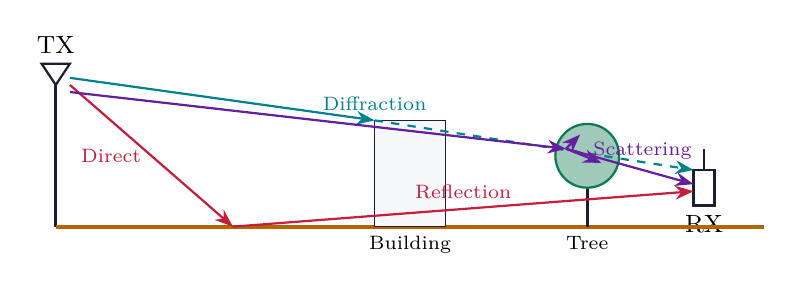
\begin{tikzpicture}[scale=0.9]
  % Transmitter tower
  \draw[line, line width=1.2pt] (0,0) -- (0,2);
  \draw[line] (0,2) -- (-0.2, 2.3) -- (0.2, 2.3) -- cycle;
  \node[above] at (0,2.3) {\small TX};

  % Receiver (Mobile)
  \draw[line, line width=1pt] (9,0.3) rectangle (9.3, 0.8);
  \draw[line] (9.15, 0.8) -- (9.15, 1.1);
  \node[below] at (9.15,0.3) {\small RX};

  % Obstacles
  % Large ground plane for reflection
  \draw[line, line width=1.5pt, color=myamber] (0,0) -- (10,0);
  
  % A sharp obstacle (building/wall) for diffraction
  \fill[draw=mydark, fill=mygray] (4.5,0) rectangle (5.5,1.5);
  \node[below, font=\scriptsize] at (5,0) {Building};

  % Scattering element (foliage/tree)
  \draw[line, line width=1pt] (7.5,0) -- (7.5,0.7);
  \draw[fill=mygreen!40, draw=mygreen, thick] (7.5,1.0) circle (0.45cm);
  \node[below, font=\scriptsize] at (7.5,0) {Tree};

  % Reflection Path
  \draw[arrow, color=myred] (0.2, 2.0) -- (2.5, 0) node[midway, left, font=\scriptsize] {Direct};
  \draw[arrow, color=myred] (2.5, 0) -- (9.0, 0.5) node[pos=0.5, above, font=\scriptsize] {Reflection};

  % Diffraction Path
  \draw[arrow, color=myteal] (0.2, 2.1) -- (4.5, 1.5);
  \draw[arrow, color=myteal, dashed] (4.5, 1.5) -- (9.0, 0.8);
  \node[above, font=\scriptsize, color=myteal] at (4.5,1.5) {Diffraction};

  % Scattering Path
  \draw[arrow, color=mypurple] (0.2, 1.9) -- (7.2, 1.1);
  \draw[arrow, color=mypurple] (7.2, 1.1) -- (7.4, 1.3);
  \draw[arrow, color=mypurple] (7.2, 1.1) -- (7.7, 0.9);
  \draw[arrow, color=mypurple] (7.2, 1.1) -- (9.0, 0.6) node[pos=0.6, above, font=\scriptsize] {Scattering};
\end{tikzpicture}
\end{tcolorbox}

% ===============================================================================
\section{Large-Scale Signal Propagation and Shadowing}
% ===============================================================================

\subsection{Path Loss and Log-Normal Shadowing}
Large-scale propagation models predict the average received signal strength over large TX-RX separation distances (hundreds or thousands of meters).
\begin{itemize}[leftmargin=*, itemsep=3.0pt]
  \item \textbf{Path Loss ($P_L$):} The attenuation of signal power as it propagates through space, modeled by:
    \begin{equation}
      P_L(d) \propto \left(\frac{d}{d_0}\right)^n
    \end{equation}
    Where $n$ is the path loss exponent and $d_0$ is a close-in reference distance.
  \item \textbf{Log-Normal Shadowing:} Represents slow fading caused by environmental obstructions (like buildings and trees) that block the line-of-sight. The received power exhibits random variations about the mean path loss, following a normal distribution when measured in decibels (dB).
\end{itemize}

\begin{tcolorbox}[formulabox, title={\textbf{Log-Normal Shadowing Model}}]
The overall path loss $P_L(d)$ in dB at distance $d$ is modeled as:
\begin{equation}
  P_L(d)[\text{dB}] = \overline{P_L}(d_0) + 10 n \log_{10}\left(\frac{d}{d_0}\right) + X_\sigma
\end{equation}
Where:
\begin{itemize}[leftmargin=*, itemsep=2pt, topsep=2pt]
  \item $\overline{P_L}(d_0) = 20\log_{10}\left(\frac{4\pi d_0}{\lambda}\right)$ is the free-space path loss at the reference distance $d_0$.
  \item $n$ is the path-loss exponent (typically 2 in free space, 3 to 5 in urban areas).
  \item $X_\sigma$ is a \textbf{zero-mean Gaussian random variable} (in dB) with standard deviation $\sigma$ (also in dB). It represents the shadowing variation.
\end{itemize}
\end{tcolorbox}

% ===============================================================================
\section{Small-Scale Fading and Multipath Parameters}
% ===============================================================================

Small-scale fading describes the rapid fluctuations of received signal amplitude and phase over very short travel distances (a few wavelengths) or short time durations.

\subsection{Multipath and Doppler Shift}
Multipath propagation occurs because the signal is reflected and scattered, arriving at the receiver via multiple paths with different amplitudes, phases, and delays.
\begin{itemize}[leftmargin=*, itemsep=3pt]
  \item \textbf{Doppler Shift ($f_d$):} The shift in received frequency due to the relative motion between the transmitter and mobile receiver:
    \begin{equation}
      f_d = \frac{v}{\lambda} \cos \theta = \frac{v \cdot f_c}{c} \cos \theta
    \end{equation}
    Where $v$ is the mobile velocity, $\lambda$ is the wavelength, $f_c$ is the carrier frequency, and $\theta$ is the arrival angle of the wave relative to the direction of motion.
\end{itemize}

\subsection{Multipath Channel Parameters}
To characterize a multipath channel, a \textbf{Power Delay Profile (PDP)} is measured by sending a short pulse and recording the received power levels at different delays ($\tau_i$).
\begin{tcolorbox}[formulabox, title={\textbf{Multipath Spread Metrics}}]
\begin{enumerate}[leftmargin=*, itemsep=4pt, label=\textbf{\arabic*.}]
  \item \textbf{Mean Excess Delay ($\overline{\tau}$):} The first moment of the power delay profile:
    \begin{equation}
      \overline{\tau} = \frac{\sum_i P(\tau_i) \tau_i}{\sum_i P(\tau_i)}
    \end{equation}
  \item \textbf{RMS Delay Spread ($\sigma_\tau$):} The square root of the second central moment of the PDP:
    \begin{equation}
      \sigma_\tau = \sqrt{\overline{\tau^2} - (\overline{\tau})^2} \quad \text{where } \overline{\tau^2} = \frac{\sum_i P(\tau_i) \tau_i^2}{\sum_i P(\tau_i)}
    \end{equation}
    \textbf{Significance:} Measures the multipath time dispersion.
  \item \textbf{Coherence Bandwidth ($B_c$):} The frequency range over which the channel passes all spectral components with equal gain and linear phase:
    \begin{equation}
      B_c \approx \frac{1}{50\sigma_\tau} \quad (\text{for } 0.9 \text{ frequency correlation}), \quad B_c \approx \frac{1}{5\sigma_\tau} \quad (\text{for } 0.5 \text{ frequency correlation})
    \end{equation}
\end{enumerate}
\end{tcolorbox}

\begin{tcolorbox}[tikzbox, title={Multipath Power Delay Profile (PDP)}]
\centering
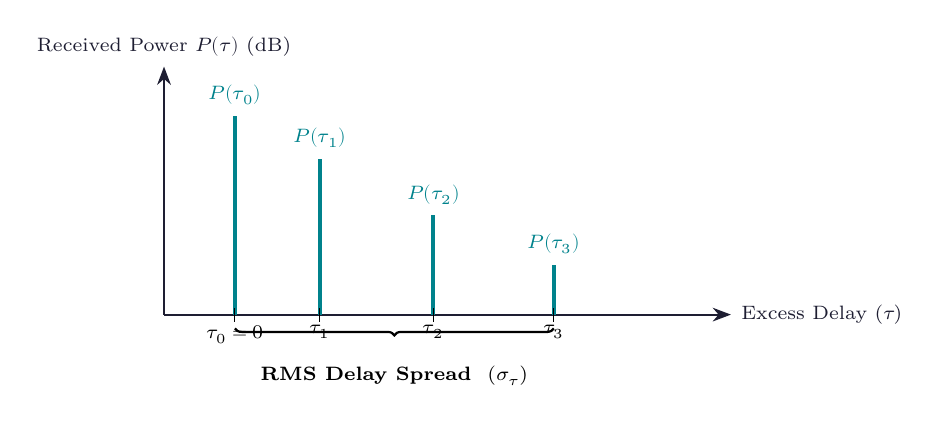
\begin{tikzpicture}[scale=0.9, every node/.style={font=\scriptsize}]
  \draw[arrow] (0,0) -- (8,0) node[right] {Excess Delay ($\tau$)};
  \draw[arrow] (0,0) -- (0,3.5) node[above] {Received Power $P(\tau)$ (dB)};

  % Multi-path spikes
  \draw[line width=1.5pt, color=myteal] (1,0) -- (1,2.8) node[above] {$P(\tau_0)$};
  \draw[line width=1.5pt, color=myteal] (2.2,0) -- (2.2,2.2) node[above] {$P(\tau_1)$};
  \draw[line width=1.5pt, color=myteal] (3.8,0) -- (3.8,1.4) node[above] {$P(\tau_2)$};
  \draw[line width=1.5pt, color=myteal] (5.5,0) -- (5.5,0.7) node[above] {$P(\tau_3)$};

  \draw (1,-0.1) -- (1,0.1) node[below=3pt] {$\tau_0=0$};
  \draw (2.2,-0.1) -- (2.2,0.1) node[below=3pt] {$\tau_1$};
  \draw (3.8,-0.1) -- (3.8,0.1) node[below=3pt] {$\tau_2$};
  \draw (5.5,-0.1) -- (5.5,0.1) node[below=3pt] {$\tau_3$};

  % Label showing delay spread
  \draw[thick, decoration={brace, mirror, raise=5pt}, decorate] (1,0) -- (5.5,0);
  \node[below=15pt] at (3.25,0) {\textbf{RMS Delay Spread } ($\sigma_\tau$)};
\end{tikzpicture}
\end{tcolorbox}

\subsection{Doppler Spread and Coherence Time}
While delay spread characterizes the time-dispersive nature of the channel, Doppler spread characterizes its time-varying nature:
\begin{itemize}[leftmargin=*, itemsep=3.0pt]
  \item \textbf{Doppler Spread ($B_D$):} The range of frequencies over which the received Doppler spectrum is non-zero. It equals the maximum Doppler shift $f_m = v/\lambda$.
  \item \textbf{Coherence Time ($T_c$):} The time duration over which the channel impulse response remains virtually constant:
    \begin{equation}
      T_c \approx \frac{9}{16\pi f_m} \approx \frac{0.178}{f_m} \quad (\text{rigorous}), \quad T_c \approx \frac{0.423}{f_m} \quad (\text{standard approximation})
    \end{equation}
\end{itemize}

% ===============================================================================
\section{Fading Classification and Channel Models}
% ===============================================================================

\subsection{Fading Classification}
Small-scale fading is classified based on two independent mechanisms: time dispersion (delay spread vs. symbol period) and frequency dispersion (Doppler spread vs. symbol rate).

\begin{tcolorbox}[tikzbox, title={Small-Scale Fading Classification Hierarchy}]
\centering
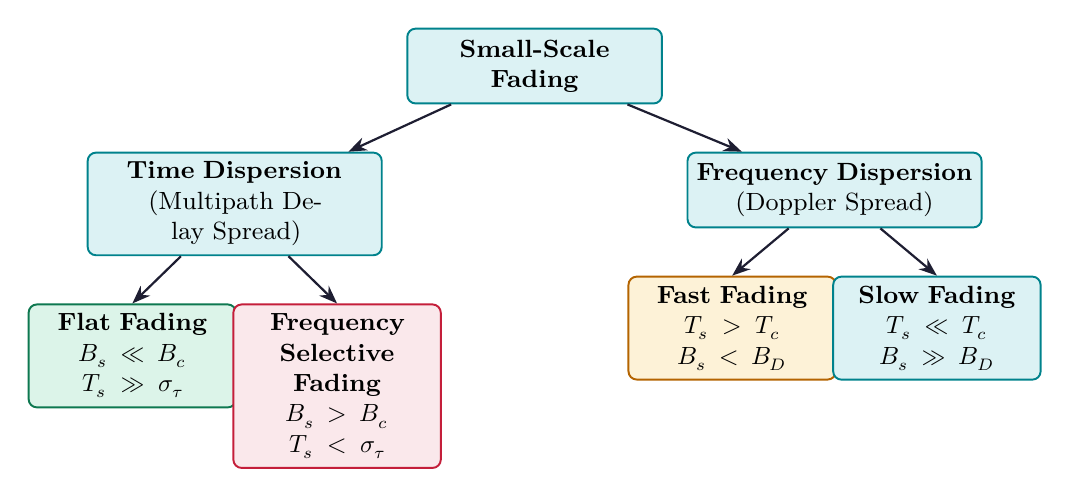
\begin{tikzpicture}[node distance=0.8cm and 0.8cm, every node/.style={font=\scriptsize}]
  \node[block, text width=3cm] (root) {\textbf{Small-Scale Fading}};
  
  \node[block, text width=3.5cm, below left=0.6cm and 0.3cm of root] (time) {\textbf{Time Dispersion}\\(Multipath Delay Spread)};
  \node[block, text width=3.5cm, below right=0.6cm and 0.3cm of root] (freq) {\textbf{Frequency Dispersion}\\(Doppler Spread)};

  \node[block, draw=mygreen, fill=hdrgreen, text width=2.4cm, below=0.6cm of time, xshift=-1.3cm] (flat) {\textbf{Flat Fading}\\$B_s \ll B_c$\\$T_s \gg \sigma_\tau$};
  \node[block, draw=myred, fill=hdrred, text width=2.4cm, below=0.6cm of time, xshift=1.3cm] (freqsel) {\textbf{Frequency\\Selective Fading}\\$B_s > B_c$\\$T_s < \sigma_\tau$};

  \node[block, draw=myamber, fill=hdramber, text width=2.4cm, below=0.6cm of freq, xshift=-1.3cm] (fast) {\textbf{Fast Fading}\\$T_s > T_c$\\$B_s < B_D$};
  \node[block, draw=myteal, fill=hdrteal, text width=2.4cm, below=0.6cm of freq, xshift=1.3cm] (slow) {\textbf{Slow Fading}\\$T_s \ll T_c$\\$B_s \gg B_D$};

  \draw[arrow] (root) -- (time);
  \draw[arrow] (root) -- (freq);
  \draw[arrow] (time) -- (flat.north);
  \draw[arrow] (time) -- (freqsel.north);
  \draw[arrow] (freq) -- (fast.north);
  \draw[arrow] (freq) -- (slow.north);
\end{tikzpicture}
\end{tcolorbox}

\subsection{Statistical Multipath Models}
When the received signal consists of multiple independent multipath waves, the envelope of the signal is modeled statistically:
\begin{enumerate}[label=\textbf{\arabic*.}, leftmargin=*, itemsep=4pt]
  \item \textbf{Rayleigh Fading (NLOS):} Used when there is no dominant line-of-sight (LOS) path. The received signal envelope $r$ is the sum of many independent scattered paths, following a Rayleigh probability density function (PDF):
    \begin{equation}
      p(r) = \frac{r}{\sigma^2} \exp\left(-\frac{r^2}{2\sigma^2}\right) \quad (r \ge 0)
    \end{equation}
    Where $\sigma^2$ is the time-average power of the received signal.
  \item \textbf{Ricean Fading (LOS):} Used when there is a dominant, direct line-of-sight (LOS) path in addition to multiple scattered paths. The envelope $r$ follows a Ricean PDF:
    \begin{equation}
      p(r) = \frac{r}{\sigma^2} \exp\left(-\frac{r^2 + A^2}{2\sigma^2}\right) I_0\left(\frac{A r}{\sigma^2}\right) \quad (r \ge 0)
    \end{equation}
    Where $A$ is the peak amplitude of the dominant LOS component, $\sigma^2$ is the variance of the scattered components, and $I_0(\cdot)$ is the modified Bessel function of the first kind of zeroth order.
  \item The channel is characterized by the \textbf{Ricean K-factor}:
    \begin{equation}
      K = \frac{\text{Power in dominant component}}{\text{Power in scattered components}} = \frac{A^2}{2\sigma^2}
    \end{equation}
    As $K \to 0$ ($-\infty$ dB), Ricean fading degenerates into Rayleigh fading. As $K \to \infty$, the channel becomes a static, fading-free LOS channel.
\end{enumerate}

\subsection{Level Crossing Rate (LCR) and Average Fade Duration (AFD)}
To design error correction codes and interleaver depths, we must know how often the signal falls below a threshold and how long it remains there:
\begin{itemize}[leftmargin=*, itemsep=3.5pt]
  \item \textbf{Level Crossing Rate (LCR, $N_R$):} The average number of times per second that the fading signal envelope crosses a specified threshold level $R$ in the positive direction:
    \begin{equation}
      N_R = \sqrt{2\pi} f_m \rho e^{-\rho^2}
    \end{equation}
    Where $f_m$ is the maximum Doppler shift and $\rho = R/R_{\text{rms}}$ is the normalized threshold level.
  \item \textbf{Average Fade Duration (AFD, $\overline{\tau}$):} The average period of time the received signal envelope remains below the threshold level $R$:
    \begin{equation}
      \overline{\tau} = \frac{e^{\rho^2} - 1}{\rho f_m \sqrt{2\pi}}
    \end{equation}
    \textbf{Significance:} AFD is inversely proportional to $f_m$. Fast-moving vehicles experience short fades, whereas slow-moving users experience long, deep fades.
\end{itemize}

% ===============================================================================
% MANDATORY QUICK REVISION PAGE
% ===============================================================================
\newpage
\begin{center}
  {\large\bfseries\color{myred} Quick Revision --- Module II}\\[3pt]
  {\small\color{mydark} Signal Propagation and Fading Channels $|$ PE-EC701C}
\end{center}
\noindent{\color{myred}\rule{\linewidth}{1.2pt}}
\vspace{4pt}

\begin{tcolorbox}[formulabox, title={\textbf{Key Formulas at a Glance}}]
\renewcommand{\arraystretch}{1.3}
\begin{tabularx}{\linewidth}{B{5.5cm} X}Log-Normal Path Loss & $P_L(d)[\text{dB}] = \overline{P_L}(d_0) + 10 n \log_{10}(d/d_0) + X_\sigma$ \\
Doppler Shift & $f_d = \frac{v}{\lambda} \cos \theta$ \\
Mean Excess Delay & $\overline{\tau} = \frac{\sum P(\tau_i) \tau_i}{\sum P(\tau_i)}$ \\
RMS Delay Spread & $\sigma_\tau = \sqrt{\overline{\tau^2} - (\overline{\tau})^2}$ \\
Coherence Bandwidth ($0.9$ corr) & $B_c \approx \frac{1}{50\sigma_\tau}$ \\
Coherence Time & $T_c \approx \frac{0.423}{f_m}$ \quad ($f_m$ = max Doppler frequency) \\
Level Crossing Rate (LCR) & $N_R = \sqrt{2\pi} f_m \rho e^{-\rho^2}$ \\
Average Fade Duration (AFD) & $\overline{\tau} = \frac{e^{\rho^2} - 1}{\rho f_m \sqrt{2\pi}}$ \\
Ricean K-factor & $K = \frac{A^2}{2\sigma^2}$ \quad ($K \to 0$ for Rayleigh fading)
\end{tabularx}
\end{tcolorbox}

\begin{tcolorbox}[defbox, title={\textbf{One-Line Definitions}}]
\begin{itemize}[leftmargin=*, itemsep=2.5pt, topsep=0pt]
  \item \textbf{Lognormal Shadowing:} Slow fading caused by obstacles in the path, causing log-normal power variations.
  \item \textbf{Knife-Edge Diffraction:} Wave bending around sharp obstacles, modeled as an infinite half-plane.
  \item \textbf{Rayleigh Fading:} Statistical model for multi-path signal envelopes with no dominant line-of-sight path.
  \item \textbf{Ricean Fading:} Statistical model for multi-path envelopes containing a dominant line-of-sight component.
  \item \textbf{Coherence Bandwidth:} Range of frequencies over which the channel has constant gain and linear phase.
  \item \textbf{Coherence Time:} Maximum time separation over which two received signals are highly correlated in phase.
  \item \textbf{Flat Fading:} Fading where the channel bandwidth is larger than the signal bandwidth ($B_c \gg B_s$).
  \item \textbf{Frequency Selective Fading:} Fading where the signal bandwidth is wider than the channel coherence bandwidth ($B_s > B_c$).
\end{itemize}
\end{tcolorbox}

\begin{tcolorbox}[exambox, title={\textbf{Frequently Asked / Viva Questions}}]
\begin{enumerate}[topsep=0pt, label=\textbf{Q\arabic*.}, itemsep=5pt]
  \item \Q{Compare reflection, diffraction, and scattering.}
    Reflection occurs at objects much larger than the wavelength $\lambda$ (ground, walls). Diffraction occurs at sharp obstacles (hills, roofs) bending waves. Scattering occurs at objects smaller than $\lambda$ (leaves, rain).
  \item \Q{What causes small-scale fading in mobile channels?}
    It is caused by the interference of multiple reflected, diffracted, and scattered waves (multipath components) arriving at the receiver with arbitrary amplitudes and phases.
  \item \Q{What is the difference between flat and frequency selective fading? How are they classified?}
    Flat fading ($T_s \gg \sigma_\tau$ or $B_s \ll B_c$) preserves the pulse shape without ISI. Frequency selective fading ($T_s < \sigma_\tau$ or $B_s > B_c$) distorts the signal, causing Inter-Symbol Interference (ISI).
  \item \Q{What is the difference between slow and fast fading?}
    Fast fading ($T_s > T_c$) causes rapid channel changes within one symbol period, distorting the pulse envelope. Slow fading ($T_s \ll T_c$) keeps the channel constant over several symbols.
  \item \Q{Explain the physical significance of the K-factor in Ricean fading.}
    It represents the ratio of the power in the line-of-sight (LOS) direct path to the total power in the scattered paths. When $K=0$, it matches Rayleigh fading.
  \item \Q{How does vehicle velocity affect coherence time and average fade duration?}
    Higher velocity increases the Doppler shift ($f_m \propto v$). Since coherence time and AFD are inversely proportional to $f_m$, higher speeds shorten both.
  \item \Q{Why do we define a reference distance $d_0$ in path loss equations?}
    The close-in reference distance $d_0$ ensures the model operates in the far-field region of the transmitter antenna, where the power law approximation is valid.
  \item \Q{Describe the power delay profile (PDP) and its application.}
    A plot of received signal power as a function of excess time delay. It is used to compute mean excess delay, RMS delay spread, and coherence bandwidth.
  \item \Q{What is the significance of the level crossing rate (LCR)?}
    It helps determine the expected rate of fading occurrences below a threshold, which is critical for choosing interleaving depths and channel coding parameters.
  \item \Q{Explain the physical cause of a Doppler shift.}
    Relative movement between the mobile station and the base station changes the path length, resulting in a shift in received frequency.
  \item \Q{Under what condition does a Ricean distribution become a Rayleigh distribution?}
    When the direct line-of-sight component becomes completely blocked, its amplitude $A \to 0$. The K-factor becomes 0, and the Ricean distribution degrades to a Rayleigh distribution.
  \item \Q{Why does frequency selective fading cause Inter-Symbol Interference (ISI)?}
    Because the channel's delay spread $\sigma_\tau$ is larger than the symbol period $T_s$. This causes energy from a preceding symbol to leak into subsequent symbols.
\end{enumerate}
\tcbset{colbacktitle=myteal, coltitle=white}
\end{tcolorbox}

\begin{tcolorbox}[tikzbox, title={Fading Types Summary Table}]
\renewcommand{\arraystretch}{1.4}
\par\noindent
{\renewcommand{\arraystretch}{1.65}%
\begin{tabularx}{\linewidth}{|B{3.0cm}|Y|Y|}\hline
\textbf{Fading Type} & \textbf{Relation} & \textbf{Primary Effect} \\
\hline
\textbf{Flat Fading} & $B_s \ll B_c$ \;/\; $T_s \gg \sigma_\tau$ & Amplitude fluctuates, pulse shape preserved. No ISI. \\[4pt]
\hline
\textbf{Freq. Selective} & $B_s > B_c$ \;/\; $T_s < \sigma_\tau$ & Signal distorted, severe ISI. Requires equalizer. \\[4pt]
\hline
\textbf{Fast Fading} & $T_s > T_c$ \;/\; $B_s < B_D$ & Channel changes within symbol. Distorts envelope. \\[4pt]
\hline
\textbf{Slow Fading} & $T_s \ll T_c$ \;/\; $B_s \gg B_D$ & Channel constant over many symbols. Normal detection. \\[4pt]
\hline
\end{tabularx}
}
\tcbset{colbacktitle=myteal, coltitle=white}
\end{tcolorbox}


% -- Module 3 -----------------------------------------------------------------
\modulestart{3}{Capacity of Wireless Fading Channels}

\section{Capacity of Wireless Fading Channels}
% ===============================================================================

Channel capacity defines the maximum error-free transmission rate achievable over a communication link. Fading causes the signal-to-noise ratio (SNR) at the receiver to fluctuate, making capacity calculations more complex than in static additive white Gaussian noise (AWGN) channels.

\subsection{Capacity of Flat Fading Channels}
In flat fading channels, the channel gain is constant across the signal bandwidth but varies over time. Let $B$ be the bandwidth, $g(t)$ be the time-varying channel power gain, $P$ be the transmit power, and $N_0$ be the noise PSD. The instantaneous SNR is:
\begin{equation}
  \gamma(t) = \frac{P \cdot g(t)}{N_0 B}
\end{equation}
The capacity depends on what Channel State Information (CSI) is available at the transmitter and receiver:

\begin{enumerate}[label=\textbf{\arabic*.}, leftmargin=*, itemsep=3.5pt]
  \item \textbf{CSI Known at Receiver Only (CSIR):} The transmitter sends data at a constant rate. The average achievable rate over time is the \textbf{Ergodic Capacity}:
    \begin{equation}
      C_{\text{ergodic}} = B \cdot \mathbb{E}\left[ \log_2(1 + \gamma) \right] = B \int_{0}^{\infty} \log_2(1 + \gamma) p(\gamma) \, d\gamma
    \end{equation}
    Where $p(\gamma)$ is the PDF of the SNR (e.g., exponential for Rayleigh fading).
  \item \textbf{CSI Known at Transmitter and Receiver (CSIT + CSIR):} The transmitter dynamically adapts its transmit power $P(\gamma)$ and data rate to match the channel state:
    \begin{equation}
      C = \max_{P(\gamma): \mathbb{E}[P(\gamma)] \le P} B \cdot \mathbb{E}\left[ \log_2\left(1 + \frac{P(\gamma)\gamma}{P}\right) \right]
    \end{equation}
    The optimal power allocation is achieved using the \textbf{water-filling algorithm}.
  \item \textbf{Outage Capacity:} If the channel changes slowly, we cannot guarantee error-free transmission at a constant rate. Outage capacity is defined as the maximum rate $C_{\text{out}}$ that can be supported with a probability of outage less than $\epsilon$:
    \begin{equation}
      P(\text{Capacity} < C_{\text{out}}) = \epsilon
    \end{equation}
\end{enumerate}

\subsection{Capacity of Frequency Selective Channels and Water-Filling}
In frequency selective fading, the channel bandwidth is larger than the coherence bandwidth ($B_s > B_c$). The channel is modeled as a set of parallel independent flat-fading subchannels (or subcarriers) using Orthogonal Frequency Division Multiplexing (OFDM).

\begin{tcolorbox}[defbox]
\textbf{Water-Filling (Water-Pouring) Algorithm:} An optimization algorithm that allocates transmit power across parallel independent communication channels to maximize total capacity under a total power constraint. It allocates more power to channels with high gains (low noise) and zero power to channels with gains below a threshold.
\end{tcolorbox}

Let the bandwidth $B$ be divided into $N$ narrow subchannels, each of width $\Delta f = B/N$. Let $\gamma_i = g_i / (N_0 \Delta f)$ be the normalized channel gain of the $i$-th subchannel. The capacity optimization problem is:
\begin{equation}
  \max_{P_i} \sum_{i=1}^{N} \Delta f \log_2\left(1 + \frac{P_i \cdot g_i}{N_0 \Delta f}\right) \quad \text{subject to } \sum_{i=1}^{N} P_i = P_{\text{total}}, \; P_i \ge 0
\end{equation}
Using Lagrange multipliers, the optimal power allocation for subchannel $i$ is:
\begin{equation}
  P_i = \left( \frac{1}{\lambda_0} - \frac{N_0 \Delta f}{g_i} \right)^{\!+}
\end{equation}
Where $\frac{1}{\lambda_0}$ is the common "water-level" and $(x)^+ = \max(x, 0)$.

\begin{tcolorbox}[tikzbox, title={Water-Filling Algorithm Concept}]
\centering
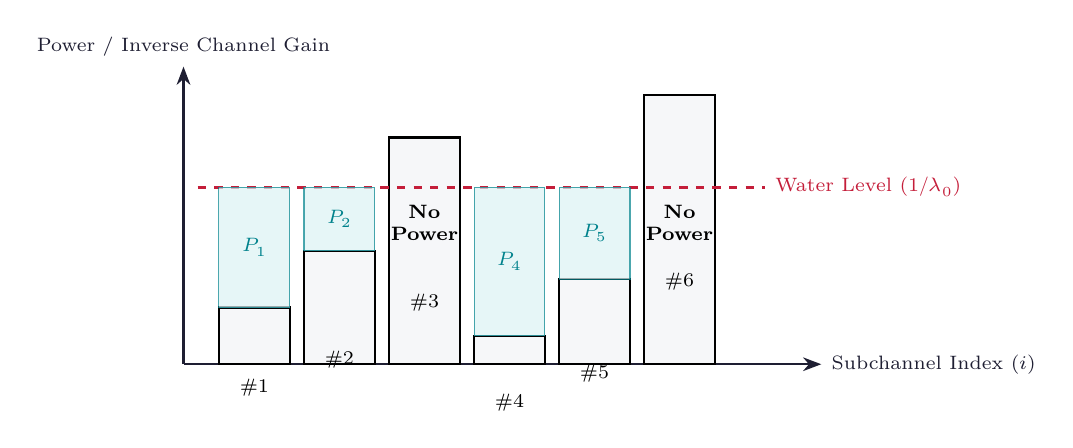
\begin{tikzpicture}[scale=0.9, every node/.style={font=\scriptsize}]
  % Draw axes
  \draw[arrow] (0,0) -- (9,0) node[right] {Subchannel Index ($i$)};
  \draw[arrow] (0,0) -- (0,4.2) node[above] {Power / Inverse Channel Gain};

  % Subchannel boxes (representing inverse gains N_0 * \Delta f / g_i)
  % Subchannel 1 (good gain, low inverse)
  \draw[thick, fill=mygray] (0.5, 0) rectangle (1.5, 0.8) node[midway, below=12pt] {\#1};
  % Subchannel 2 (moderate)
  \draw[thick, fill=mygray] (1.7, 0) rectangle (2.7, 1.6) node[midway, below=12pt] {\#2};
  % Subchannel 3 (poor, high inverse)
  \draw[thick, fill=mygray] (2.9, 0) rectangle (3.9, 3.2) node[midway, below=12pt] {\#3};
  % Subchannel 4 (excellent, lowest inverse)
  \draw[thick, fill=mygray] (4.1, 0) rectangle (5.1, 0.4) node[midway, below=12pt] {\#4};
  % Subchannel 5 (moderate)
  \draw[thick, fill=mygray] (5.3, 0) rectangle (6.3, 1.2) node[midway, below=12pt] {\#5};
  % Subchannel 6 (very bad, above water level)
  \draw[thick, fill=mygray] (6.5, 0) rectangle (7.5, 3.8) node[midway, below=12pt] {\#6};

  % Water Level line
  \draw[dashed, color=myred, line width=1.1pt] (0.2, 2.5) -- (8.2, 2.5) node[right, color=myred] {Water Level ($1/\lambda_0$)};

  % Allocated Power (Water) filling the bins up to the water level
  \fill[draw=myteal, fill=hdrteal, opacity=0.7] (0.5, 0.8) rectangle (1.5, 2.5);
  \node at (1, 1.65) {\color{myteal}\textbf{$P_1$}};
  
  \fill[draw=myteal, fill=hdrteal, opacity=0.7] (1.7, 1.6) rectangle (2.7, 2.5);
  \node at (2.2, 2.05) {\color{myteal}\textbf{$P_2$}};

  \fill[draw=myteal, fill=hdrteal, opacity=0.7] (4.1, 0.4) rectangle (5.1, 2.5);
  \node at (4.6, 1.45) {\color{myteal}\textbf{$P_4$}};

  \fill[draw=myteal, fill=hdrteal, opacity=0.7] (5.3, 1.2) rectangle (6.3, 2.5);
  \node at (5.8, 1.85) {\color{myteal}\textbf{$P_5$}};

  % Label for unallocated bin #3 and #6
  \node[align=center] at (3.4, 2.0) {\textbf{No}\\\textbf{Power}};
  \node[align=center] at (7.0, 2.0) {\textbf{No}\\\textbf{Power}};
\end{tikzpicture}
\end{tcolorbox}

% ===============================================================================
\section{Antennas for Mobile Terminals}
% ===============================================================================

Mobile terminal antennas must be compact, lightweight, and low-profile to fit within handheld devices while maintaining high radiation efficiency over multiple operating bands.

\subsection{Monopole Antennas}
A monopole antenna consists of a straight rod-shaped conductor mounted perpendicularly over a conducting ground plane.
\begin{itemize}[leftmargin=*, itemsep=3pt]
  \item \textbf{Working Principle:} When fed at its base, the antenna forms a resonant structure. By electromagnetic imaging theory, the conducting ground plane creates a virtual image of the monopole, causing it to behave like a half-wave ($\lambda/2$) dipole.
  \item \textbf{Length:} The standard physical length is a quarter-wavelength ($\lambda/4$).
  \item \textbf{Radiation Pattern:} Omnidirectional in the azimuth plane (horizontal), with a toroidal (donut-shaped) pattern in 3D.
  \item \textbf{Limitations:} Its vertical protrusion makes it unsuitable for modern, ultra-thin smartphones.
\end{itemize}

\subsection{Planar Inverted-F Antenna (PIFA)}
The PIFA is the dominant antenna technology for modern smartphones. It is derived from a conventional rectangular patch antenna by shorting the radiating patch to the ground plane at one end.

\begin{tcolorbox}[defbox]
\textbf{Planar Inverted-F Antenna (PIFA):} A low-profile, space-saving antenna consisting of a rectangular radiating patch suspended parallel to a ground plane, fed by a coaxial probe, and shorted to the ground plane at one edge using a shorting plate or pin. The shorting pin reduces the resonant length of the patch from $\lambda/2$ to $\lambda/4$.
\end{tcolorbox}

\begin{itemize}[leftmargin=*, itemsep=2.5pt]
  \item \textbf{Geometry:} The feed point is placed near the shorting pin. Adjusting the distance between the feed point and the shorting pin controls the input impedance, allowing easy matching to $50\,\Omega$ without external components.
  \item \textbf{Resonant Frequency Formula:} The approximate resonant frequency for a rectangular PIFA is:
    \begin{equation}
      f_r \approx \frac{c}{4(W + L)}
    \end{equation}
    Where $L$ and $W$ are the length and width of the radiating patch, and $c$ is the speed of light.
  \item \textbf{Advantages:} Ultra-low profile, easy to embed within device casings, reduced radiation toward the user's head (due to the shielding effect of the ground plane), and support for multi-band operation by slotting the patch.
\end{itemize}

\begin{tcolorbox}[tikzbox, title={Planar Inverted-F Antenna (PIFA) Structure}]
\centering
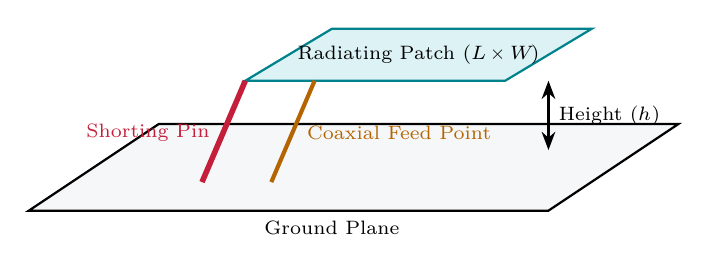
\begin{tikzpicture}[scale=1.1, every node/.style={font=\scriptsize}]
  % Draw Ground Plane (Base)
  \draw[thick, fill=mygray] (0,0) -- (6,0) -- (7.5,1) -- (1.5,1) -- cycle;
  \node[below] at (3.5,0) {Ground Plane};

  % Draw Radiating Patch (Suspended)
  \draw[thick, fill=hdrteal, draw=myteal] (2.5,1.5) -- (5.5,1.5) -- (6.5,2.1) -- (3.5,2.1) -- cycle;
  \node at (4.5, 1.8) {Radiating Patch ($L \times W$)};

  % Draw Shorting Wall/Pin
  \draw[line width=2pt, color=myred] (2.5,1.5) -- (2.0, 0.33);
  \node[left, color=myred] at (2.2, 0.9) {Shorting Pin};

  % Draw Feed Pin
  \draw[line width=1.5pt, color=myamber] (3.3,1.5) -- (2.8, 0.33);
  \node[right, color=myamber] at (3.1, 0.9) {Coaxial Feed Point};

  % Height indication
  \draw[Stealth-Stealth, thick] (6.0, 1.5) -- (6.0, 0.7) node[midway, right] {Height ($h$)};
\end{tikzpicture}
\end{tcolorbox}

% ===============================================================================
\section{Base Station Antennas and Arrays}
% ===============================================================================

Base station antennas must handle high RF power, shape radiation beams to cover specific geographic sectors, and dynamically adapt to user distribution.

\subsection{Omnidirectional vs. Sectorized Antennas}
\begin{itemize}[leftmargin=*, itemsep=3.5pt]
  \item \textbf{Omnidirectional Antennas:} Radiate power equally in all horizontal directions. Used in low-density rural areas or microcells with central base stations.
  \item \textbf{Sectorized Antennas:} Use directional antennas (typically panel antennas containing array dipoles) to concentrate radiation into a specific sector.
    \begin{itemize}[leftmargin=*, itemsep=2pt, topsep=2pt]
      \item \textbf{3-Sector Configuration:} 3 antennas, each covering a $120^\circ$ beamwidth (half-power beamwidth - HPBW).
      \item \textbf{6-Sector Configuration:} 6 antennas, each covering a $60^\circ$ beamwidth. Reduces co-channel interference, boosting network capacity.
    \end{itemize}
\end{itemize}

\begin{tcolorbox}[tikzbox, title={Base Station Sectorization Patterns}]
\centering
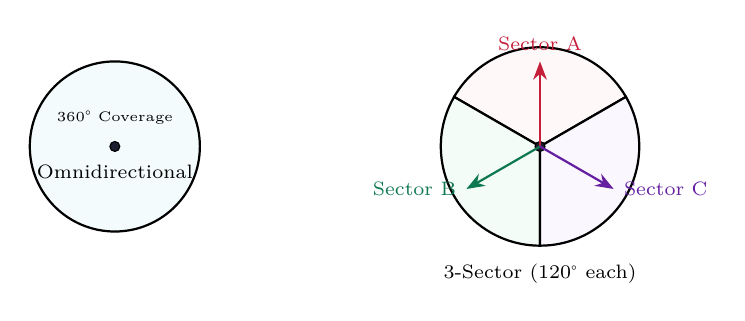
\begin{tikzpicture}[scale=0.9, every node/.style={font=\scriptsize}]
  % Omnidirectional cell (Circle)
  \draw[thick, fill=hdrteal!30] (-3,0) circle (1.2cm);
  \draw[fill=mydark] (-3,0) circle (2pt);
  \node[below=3pt] at (-3,0) {Omnidirectional};
  \node[font=\tiny] at (-3, 0.4) {360$^\circ$ Coverage};

  % Sectorized cell (3 Sectors of 120 degrees)
  \begin{scope}[shift={(3,0)}]
    \draw[thick, fill=hdrred!30] (0,0) -- (30:1.4) arc (30:150:1.4) -- cycle;
    \draw[thick, fill=hdrgreen!30] (0,0) -- (150:1.4) arc (150:270:1.4) -- cycle;
    \draw[thick, fill=hdrpurple!30] (0,0) -- (270:1.4) arc (270:390:1.4) -- cycle;
    \draw[fill=mydark] (0,0) circle (2pt);
    \node[below=3pt] at (0,-1.4) {3-Sector ($120^\circ$ each)};
    \draw[arrow, redarrow] (0,0) -- (90:1.2) node[above] {Sector A};
    \draw[arrow, color=mygreen] (0,0) -- (210:1.2) node[left] {Sector B};
    \draw[arrow, color=mypurple] (0,0) -- (330:1.2) node[right] {Sector C};
  \end{scope}
\end{tikzpicture}
\end{tcolorbox}

\subsection{Smart Antennas}
Smart antennas combine multiple antenna elements with digital signal processing to dynamically optimize the radiation pattern:
\begin{enumerate}[label=\textbf{\arabic*.}, leftmargin=*, itemsep=3.5pt]
  \item \textbf{Switched-Beam Antennas:} Feature a collection of fixed, directional beams. The system detects the user's signal strength and switches to the beam that provides the best alignment. It is simple but cannot track users continuously.
  \item \textbf{Adaptive Array Antennas:} Continuously adjust amplitude and phase weights (beamforming) to dynamically steer the main lobe of the antenna pattern toward the desired user while placing nulls in the direction of interferers.
\end{enumerate}

\subsection{Antenna Arrays}
An antenna array is a spatial arrangement of multiple antenna elements (usually dipoles or patches) fed with controlled phase and amplitude shifts:
\begin{itemize}[leftmargin=*, itemsep=3pt]
  \item \textbf{Array Factor ($AF$):} For a linear array of $M$ elements spaced at distance $d$:
    \begin{equation}
      AF(\theta) = \sum_{m=0}^{M-1} a_m e^{j m (k d \cos\theta + \beta)}
    \end{equation}
    Where $a_m$ is the amplitude weight, $k = 2\pi/\lambda$ is the wave number, $\beta$ is the progressive phase shift, and $\theta$ is the angle relative to the array axis.
  \item By adjusting $\beta$, the main beam can be steered electronically (\textbf{phased arrays}) without physically moving the antenna.
\end{itemize}

% ===============================================================================
% MANDATORY QUICK REVISION PAGE
% ===============================================================================
\newpage
\begin{center}
  {\large\bfseries\color{myred} Quick Revision --- Module III}\\[3pt]
  {\small\color{mydark} Channel Capacity and Mobile Antennas $|$ PE-EC701C}
\end{center}
\noindent{\color{myred}\rule{\linewidth}{1.2pt}}
\vspace{4pt}

\begin{tcolorbox}[formulabox, title={\textbf{Key Formulas at a Glance}}]
\renewcommand{\arraystretch}{1.3}
\begin{tabularx}{\linewidth}{B{5.5cm} X}AWGN Channel Capacity & $C = B \log_2(1 + \text{SNR})$ \\
Ergodic Capacity (CSIR only) & $C = B \cdot \mathbb{E}\left[ \log_2(1 + \gamma) \right]$ \\
Water-Filling Power Allocation & $P_i = \left( \frac{1}{\lambda_0} - \frac{N_0 \Delta f}{g_i} \right)^{\!+}$ \quad ($\sum P_i = P_{\text{total}}$) \\
Outage Probability & $P_{\text{out}} = P(C(\gamma) < R)$ \\
PIFA Resonant Frequency & $f_r \approx \frac{c}{4(W + L)}$ \\
Monopole Resonant Length & $L \approx \frac{\lambda}{4}$ \\
Array Factor (Linear Array) & $AF(\theta) = \sum_{m=0}^{M-1} a_m e^{j m (k d \cos\theta + \beta)}$
\end{tabularx}
\end{tcolorbox}

\begin{tcolorbox}[defbox, title={\textbf{One-Line Definitions}}]
\begin{itemize}[leftmargin=*, itemsep=2.5pt, topsep=0pt]
  \item \textbf{Ergodic Capacity:} The long-term average transmission rate supported by a fast-fading channel.
  \item \textbf{Outage Capacity:} The maximum constant rate supported by a channel with a given outage probability threshold $\epsilon$.
  \item \textbf{Water-Filling:} An optimal power allocation strategy that prioritizes channels with high gains (low noise).
  \item \textbf{PIFA:} Planar Inverted-F Antenna, a compact, low-profile internal antenna used in mobile phones.
  \item \textbf{Monopole Antenna:} A resonant vertical rod antenna fed above a conducting ground plane.
  \item \textbf{Adaptive Array:} An antenna array that dynamically steers its beam toward the user and places nulls toward interferers.
  \item \textbf{Beamforming:} Shifting the phase and amplitude of array elements to create constructive interference in a desired direction.
\end{itemize}
\end{tcolorbox}

\begin{tcolorbox}[exambox, title={\textbf{Frequently Asked / Viva Questions}}]
\begin{enumerate}[topsep=0pt, label=\textbf{Q\arabic*.}, itemsep=5pt]
  \item \Q{Explain the physical meaning of the water-filling algorithm.}
    It mimics pouring a fixed volume of water (representing total power) into a vessel with an uneven bottom (representing inverse channel gains). The water fills the deepest valleys first, allocating more power to clean subchannels and no power to noisy ones.
  \item \Q{Why does a PIFA have a resonant length of $\lambda/4$ while a patch antenna requires $\lambda/2$?}
    Adding a shorting pin at the zero-electric-field boundary of a patch antenna enforces a short circuit. This changes the boundary condition, allowing the patch to resonate at a quarter-wavelength instead of a half-wavelength.
  \item \Q{Compare ergodic capacity and outage capacity.}
    Ergodic capacity represents the average rate supported over time in fast-fading channels. Outage capacity is used in slow-fading channels, representing the rate that can be guaranteed for $(1-\epsilon)\%$ of the time.
  \item \Q{What are the functions of the shorting pin and feed point in a PIFA?}
    The shorting pin forces a zero-voltage boundary condition, reducing the required physical size. Placing the feed point near the shorting pin allows the input impedance to be matched to $50\,\Omega$.
  \item \Q{Why are omnidirectional antennas not preferred at base stations in dense urban areas?}
    Omnidirectional antennas radiate power in all directions, causing high co-channel interference to adjacent cells. Sectorized antennas focus radiation, reducing co-channel interference.
  \item \Q{What is the difference between a switched-beam antenna and an adaptive array?}
    A switched-beam antenna switches between pre-configured, fixed directional beams. An adaptive array continuously calculates optimal weights to steer the main beam and nulls in real-time.
  \item \Q{What is the purpose of using antenna arrays at base stations?}
    To increase antenna gain, steer the radiation beam electronically (phased arrays), and enable spatial division multiple access (SDMA) and MIMO.
  \item \Q{State the resonant frequency approximation formula for a PIFA.}
    $f_r \approx \frac{c}{4(W+L)}$, where $L$ and $W$ are the length and width of the radiating plate, and $c$ is the velocity of light.
  \item \Q{Why is a monopole antenna modeled as a dipole over a ground plane?}
    According to the electromagnetic image theory, a conducting ground plane creates a virtual image of the vertical monopole below the plane, acting as the second half of a dipole.
  \item \Q{What is the impact of placing the feed point close to the shorting pin in PIFA?}
    As the feed point moves closer to the shorting pin, the input impedance decreases toward zero. This allows the input impedance to be matched to $50\,\Omega$.
  \item \Q{Explain how electronic beam steering is achieved in antenna arrays.}
    By introducing a progressive phase shift $\beta$ between adjacent antenna elements. This shifts the direction where the signals add constructively, steering the beam without physical rotation.
  \item \Q{Under what conditions does the water-filling algorithm allocate zero power to a subchannel?}
    When the subchannel's normalized noise-to-gain ratio ($N_0 \Delta f / g_i$) is higher than the calculated water-level threshold ($1/\lambda_0$).
\end{enumerate}
\tcbset{colbacktitle=myteal, coltitle=white}
\end{tcolorbox}

\begin{tcolorbox}[tikzbox, title={Comparison of Monopole and PIFA Antennas}]
\renewcommand{\arraystretch}{1.4}
\par\noindent
{\renewcommand{\arraystretch}{1.55}%
\begin{tabularx}{\linewidth}{|B{3.0cm}|Y|Y|}\hline
\textbf{Parameter} & \textbf{\color{myteal}Monopole Antenna} & \textbf{\color{myred}Planar Inverted-F (PIFA)} \\[4pt]
\hline
\textbf{Structure} & Simple vertical rod over a ground plane. & Flat rectangular patch parallel to a ground plane with a shorting pin. \\[4pt]
\hline
\textbf{Resonant Length} & $\lambda/4$ (vertical height). & $\approx \lambda/4$ (sum of length and width, $L+W$). \\[4pt]
\hline
\textbf{Profile} & High profile (protruding structure). & Low profile, easily embedded inside devices. \\[4pt]
\hline
\textbf{SAR (Radiation towards head)} & High (radiates symmetrically around the rod). & Low (ground plane acts as an electromagnetic shield). \\[4pt]
\hline
\end{tabularx}
}
\tcbset{colbacktitle=myteal, coltitle=white}
\end{tcolorbox}


% -- Module 4 -----------------------------------------------------------------
\modulestart{4}{Multiple Access Schemes}

\section{Multiple Access Schemes}
% ===============================================================================

Multiple access schemes allow many mobile users to share the same physical radio spectrum simultaneously without causing mutual interference.

\subsection{FDMA, TDMA, CDMA, and SDMA}
\begin{itemize}[leftmargin=*, itemsep=3.5pt]
  \item \textbf{FDMA (Frequency Division Multiple Access):} Divides the allocated spectrum into narrow, non-overlapping frequency channels. Each user is assigned a unique channel for the duration of the call. Requires guard bands to prevent adjacent channel interference. Used in 1G systems.
  \item \textbf{TDMA (Time Division Multiple Access):} Divides a single carrier frequency channel into multiple non-overlapping time slots. Each user is assigned a specific slot periodically, transmitting in bursts. Requires guard times to prevent slot overlaps. Used in GSM (2G).
  \item \textbf{CDMA (Code Division Multiple Access):} Users share the entire allocated bandwidth simultaneously. Each user's signal is multiplied by a unique, orthogonal pseudo-noise (PN) code. The receiver uses the same code to despread and recover the desired signal while treating other users' signals as wideband noise. Used in IS-95 (2G) and WCDMA (3G).
  \item \textbf{SDMA (Spatial Division Multiple Access):} Serves different users on the same frequency and time by using highly directional smart antennas (beamforming) to separate signals spatially.
\end{itemize}

\begin{tcolorbox}[tikzbox, title={TDMA Frame and Slot Structure}]
\centering
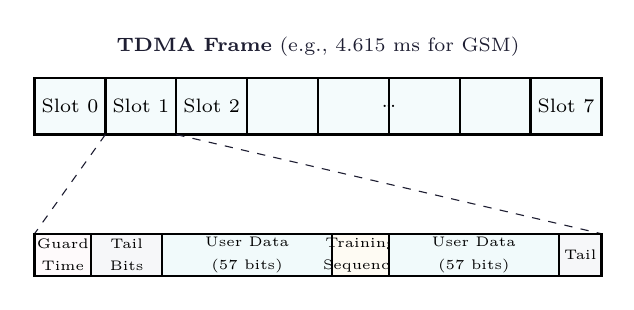
\begin{tikzpicture}[scale=0.9, every node/.style={font=\scriptsize}]
  % Draw TDMA Frame
  \draw[thick, fill=hdrteal!30] (0,1.2) rectangle (8,2.0);

  % Split slots
  \foreach \x in {1,2,3,4,5,6,7} {
    \draw[thick] (\x,1.2) -- (\x,2.0);
  }
  \node at (0.5, 1.6) {Slot 0};
  \node at (1.5, 1.6) {Slot 1};
  \node at (2.5, 1.6) {Slot 2};
  \node at (7.5, 1.6) {Slot 7};
  \node at (5.0, 1.6) {\dots};

  % Frame Label above
  \node[above=0.15cm, color=mydark] at (4, 2.0) {\textbf{TDMA Frame} (e.g., 4.615 ms for GSM)};

  % Expand Slot 1
  \draw[dashed, color=mydark] (1.0, 1.2) -- (0, -0.2);
  \draw[dashed, color=mydark] (2.0, 1.2) -- (8.0, -0.2);

  % Detail Slot structure
  \draw[thick, fill=hdrred!20] (0,-0.2) rectangle (0.8,-0.8) node[midway, align=center] {\tiny Guard\\ \tiny Time};
  \draw[thick, fill=mygray] (0.8,-0.2) rectangle (1.8,-0.8) node[midway, align=center] {\tiny Tail\\ \tiny Bits};
  \draw[thick, fill=hdrteal!40] (1.8,-0.2) rectangle (4.2,-0.8) node[midway, align=center] {\tiny User Data\\ \tiny (57 bits)};
  \draw[thick, fill=hdramber!30] (4.2,-0.2) rectangle (5.0,-0.8) node[midway, align=center] {\tiny Training\\ \tiny Sequence};
  \draw[thick, fill=hdrteal!40] (5.0,-0.2) rectangle (7.4,-0.8) node[midway, align=center] {\tiny User Data\\ \tiny (57 bits)};
  \draw[thick, fill=mygray] (7.4,-0.2) rectangle (8.0,-0.8) node[midway, align=center] {\tiny Tail};
\end{tikzpicture}
\end{tcolorbox}

% ===============================================================================
\section{Modulation Schemes in Mobile Communications}
% ===============================================================================

Mobile radio channels require modulation schemes that are spectrally efficient, robust against multipath distortion, and power efficient (low peak-to-average power ratio).

\subsection{BPSK, QPSK, and Variants}
\begin{itemize}[leftmargin=*, itemsep=3.0pt]
  \item \textbf{BPSK (Binary Phase Shift Keying):} Maps 1 bit per symbol to phases $0$ and $\pi$. Simple and robust, but has low spectral efficiency ($1\,\text{bps/Hz}$).
  \item \textbf{QPSK (Quadrature Phase Shift Keying):} Maps 2 bits per symbol to four phases ($45^\circ$, $135^\circ$, $225^\circ$, $315^\circ$). Achieves double the spectral efficiency of BPSK ($2\,\text{bps/Hz}$) within the same bandwidth.
  \item \textbf{OQPSK (Offset QPSK):} Introduces a $T_s/2$ time delay between the in-phase ($I$) and quadrature ($Q$) bit streams. This prevents simultaneous transitions of both streams, limiting phase changes to a maximum of $90^\circ$ (instead of $180^\circ$ in standard QPSK). This reduces envelope fluctuations after filtering, allowing efficient non-linear amplifiers.
  \item \textbf{$\pi/4$-DQPSK (Differential QPSK):} The phase constellation rotates by $\pi/4$ every symbol interval. The maximum phase change is limited to $135^\circ$, which prevents the signal envelope from passing through zero. This reduces spectral regrowth and simplifies demodulation using differential detection.
\end{itemize}

\subsection{MSK and GMSK}
Non-constant envelope signals experience severe distortion when passed through non-linear power amplifiers. Constant envelope modulation schemes solve this issue:
\begin{itemize}[leftmargin=*, itemsep=3pt]
  \item \textbf{MSK (Minimum Shift Keying):} A continuous-phase frequency shift keying (CPFSK) scheme with a modulation index $m = 0.5$ (minimum frequency spacing for orthogonal detection). The phase changes linearly over each symbol period.
  \item \textbf{GMSK (Gaussian Minimum Shift Keying):} Derived from MSK by filtering the baseband NRZ data stream through a Gaussian low-pass filter before frequency modulation.
    \begin{itemize}[leftmargin=*, itemsep=2pt, topsep=2pt]
      \item \textbf{Advantage:} The Gaussian filter smooths the phase transitions, suppressing the side lobes of the transmitted spectrum. This minimizes adjacent channel interference (ACI).
      \item \textbf{Trade-off:} The smoothing introduces controlled Inter-Symbol Interference (ISI) in the time domain, requiring an equalizer at the receiver. Used in the GSM standard.
    \end{itemize}
\end{itemize}

\begin{tcolorbox}[tikzbox, title={GMSK Transmitter Block Diagram}]
\centering

\begin{tikzpicture}[node distance=0.6cm and 1.2cm]
  \node[block, text width=2.2cm] (data) {\textbf{Digital Data}\\(NRZ Bit Stream)};
  \node[block, right=1.2cm of data, text width=2.5cm] (gauss) {\textbf{Gaussian LPF}\\(Pulse Shaping)};
  \node[block, right=1.2cm of gauss, text width=2.2cm] (mod) {\textbf{FM Modulator}\\(VCO)};
  \node[right=1.0cm of mod] (out) {\small GMSK Output};
  
  \draw[arrow] (data) -- (gauss) node[midway, above] {$d(t)$};
  \draw[arrow] (gauss) -- (mod) node[midway, above] {$p(t)$};
  \draw[arrow] (mod) -- (out);
\end{tikzpicture}
\end{tcolorbox}

% ===============================================================================
\section{Multicarrier Modulation and OFDM}
% ===============================================================================

\subsection{Basic Principles of OFDM}
Orthogonal Frequency Division Multiplexing (OFDM) is a multicarrier modulation scheme that divides a high-speed data stream into multiple parallel, low-speed streams modulated onto orthogonal subcarriers.

\begin{tcolorbox}[defbox]
\textbf{Subcarrier Orthogonality:} Two subcarriers are orthogonal if their frequencies are spaced at multiples of the inverse of the symbol duration ($1/T$). Mathematically:
\begin{equation}
  \frac{1}{T}\int_{0}^{T} e^{j 2\pi f_m t} \cdot e^{-j 2\pi f_n t} \, dt = 0 \quad (\text{for } f_m - f_n = \frac{k}{T}, \; k \neq 0)
\end{equation}
This allows their spectra to overlap in the frequency domain without causing mutual interference (ICI), maximizing spectral efficiency.
\end{tcolorbox}

\subsection{Mathematical Formulation (IFFT/FFT Relation)}
An OFDM symbol is generated in the digital domain using the Inverse Fast Fourier Transform (IFFT). Let $X_k$ be the complex modulation symbol (e.g., QAM) mapped to the $k$-th subcarrier. The discrete-time baseband OFDM signal is:
\begin{equation}
  x(n) = \frac{1}{\sqrt{N}} \sum_{k=0}^{N-1} X_k e^{j \frac{2\pi k n}{N}} \quad \implies \text{IDFT / IFFT operation}
\end{equation}
At the receiver, the symbols are recovered using the Fast Fourier Transform (FFT):
\begin{equation}
  X_k = \frac{1}{\sqrt{N}} \sum_{n=0}^{N-1} x(n) e^{-j \frac{2\pi k n}{N}} \quad \implies \text{DFT / FFT operation}
\end{equation}

\subsection{Cyclic Prefix (CP) Insertion}
To eliminate Inter-Symbol Interference (ISI) caused by multipath delay spread, a \textbf{Cyclic Prefix (CP)} is appended to the beginning of each OFDM symbol.
\begin{itemize}[leftmargin=*, itemsep=3.0pt]
  \item \textbf{Mechanism:} The CP is a copy of the end portion of the OFDM symbol, prepended to the start. The duration of the CP ($T_{\text{CP}}$) must be longer than the maximum delay spread of the channel ($\tau_{\text{max}}$).
  \item \textbf{Purpose:} 
    \begin{itemize}[leftmargin=*, itemsep=2pt, topsep=2pt]
      \item Acts as a guard time, preventing the preceding symbol's multipath components from interfering with the current symbol (eliminates ISI).
      \item Converts linear channel convolution into circular convolution, allowing simple one-tap frequency-domain equalization (FDE) at the receiver.
    \end{itemize}
\end{itemize}

\subsection{Peak-to-Average Power Ratio (PAPR) Issue}
The primary drawback of OFDM is its high PAPR.
\begin{itemize}[leftmargin=*, itemsep=3.5pt]
  \item \textbf{Cause:} Because an OFDM symbol is the sum of many independent subcarriers, their constructive phase alignment can produce large peak signals relative to the average power.
  \item \textbf{Impact:} High PAPR requires power amplifiers with wide linear ranges, reducing efficiency and increasing costs. Non-linear amplification causes out-of-band emissions and in-band distortion.
  \item \textbf{Mitigation:} Clipping and filtering, selective mapping (SLM), coding (e.g., Golay complementary sequences), and using Single-Carrier FDMA (SC-FDMA) on the uplink (as in LTE).
\end{itemize}

\begin{tcolorbox}[tikzbox, title={OFDM Transmitter and Receiver Block Diagrams}]
\centering
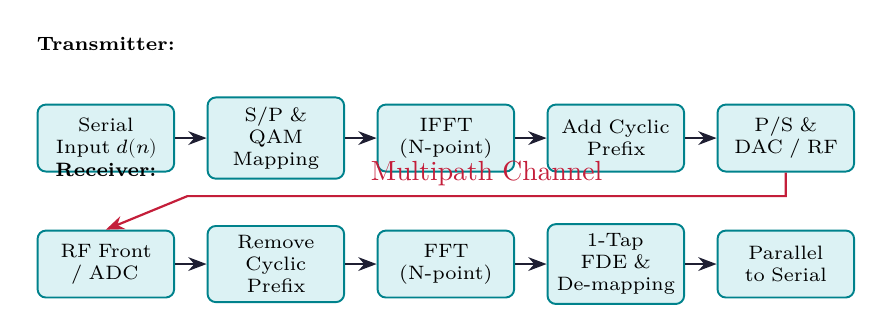
\begin{tikzpicture}[node distance=0.35cm and 0.55cm,
  sblock/.style={rectangle, draw=myteal, fill=hdrteal, text width=1.5cm,
    align=center, minimum height=0.85cm, font=\scriptsize,
    rounded corners=3pt, line width=0.7pt}]

  % Transmitter
  \node[font=\scriptsize\bfseries] at (0,1.2) {Transmitter:};
  \node[sblock] (tx_in) {Serial Input $d(n)$};
  \node[sblock, right=0.4cm of tx_in] (tx_s2p) {S/P \& QAM Mapping};
  \node[sblock, right=0.4cm of tx_s2p] (tx_ifft) {IFFT\\(N-point)};
  \node[sblock, right=0.4cm of tx_ifft] (tx_cp) {Add Cyclic Prefix};
  \node[sblock, right=0.4cm of tx_cp] (tx_p2s) {P/S \& DAC / RF};
  \draw[arrow] (tx_in) -- (tx_s2p);
  \draw[arrow] (tx_s2p) -- (tx_ifft);
  \draw[arrow] (tx_ifft) -- (tx_cp);
  \draw[arrow] (tx_cp) -- (tx_p2s);

  % Receiver
  \node[font=\scriptsize\bfseries] at (0,-0.4) {Receiver:};
  \begin{scope}[shift={(0,-1.6)}]
    \node[sblock] (rx_in) {RF Front / ADC};
    \node[sblock, right=0.4cm of rx_in] (rx_cp) {Remove Cyclic Prefix};
    \node[sblock, right=0.4cm of rx_cp] (rx_fft) {FFT\\(N-point)};
    \node[sblock, right=0.4cm of rx_fft] (rx_eq) {1-Tap FDE \& De-mapping};
    \node[sblock, right=0.4cm of rx_eq] (rx_out) {Parallel to Serial};
    \draw[arrow] (rx_in) -- (rx_cp);
    \draw[arrow] (rx_cp) -- (rx_fft);
    \draw[arrow] (rx_fft) -- (rx_eq);
    \draw[arrow] (rx_eq) -- (rx_out);
  \end{scope}

  % Connect Tx to Rx
  \draw[arrow, redarrow] (tx_p2s.south) -- +(0,-0.3) -- node[midway, above, color=myred] {Multipath Channel} +(-7.6,-0.3) -- (rx_in.north);
\end{tikzpicture}
\end{tcolorbox}

% ===============================================================================
% MANDATORY QUICK REVISION PAGE
% ===============================================================================
\newpage
\begin{center}
  {\large\bfseries\color{myred} Quick Revision --- Module IV}\\[3pt]
  {\small\color{mydark} Multiple Access and Modulation Schemes $|$ PE-EC701C}
\end{center}
\noindent{\color{myred}\rule{\linewidth}{1.2pt}}
\vspace{4pt}

\begin{tcolorbox}[formulabox, title={\textbf{Key Formulas at a Glance}}]
\renewcommand{\arraystretch}{1.3}
\begin{tabularx}{\linewidth}{B{5.5cm} X}Subcarrier Frequency Spacing & $\Delta f = \frac{1}{T}$ \quad ($T$ = active OFDM symbol duration) \\
OFDM Subcarrier Orthogonality & $\frac{1}{T}\int_{0}^{T} e^{j 2\pi f_m t} \cdot e^{-j 2\pi f_n t} \, dt = 0 \quad (f_m - f_n = \frac{k}{T})$ \\
Discrete OFDM Signal (IFFT) & $x(n) = \frac{1}{\sqrt{N}} \sum_{k=0}^{N-1} X_k e^{j \frac{2\pi k n}{N}}$ \\
Cyclic Prefix Condition & $T_{\text{CP}} \ge \tau_{\text{max}}$ \quad ($\tau_{\text{max}}$ = max channel delay spread) \\
Peak-to-Average Power Ratio & $\text{PAPR} = \frac{\max |x(t)|^2}{\mathbb{E}[|x(t)|^2]}$ \\
MSK Frequency Separation & $\Delta f_{\text{min}} = \frac{1}{2T_b}$ \quad (minimum for coherent orthogonality)
\end{tabularx}
\end{tcolorbox}

\begin{tcolorbox}[defbox, title={\textbf{One-Line Definitions}}]
\begin{itemize}[leftmargin=*, itemsep=2.5pt, topsep=0pt]
  \item \textbf{FDMA:} Allocates unique, narrow frequency bands to users for the duration of the call.
  \item \textbf{TDMA:} Divides the carrier frequency into periodic time slots, assigning one to each user.
  \item \textbf{CDMA:} Allows users to share the entire bandwidth simultaneously using unique orthogonal codes.
  \item \textbf{Offset QPSK:} A QPSK variant that delays the Q-channel by half a symbol period to prevent envelope drops.
  \item \textbf{GMSK:} A continuous-phase modulation scheme that shapes baseband pulses using a Gaussian filter before modulation.
  \item \textbf{OFDM:} A multicarrier modulation scheme dividing a high-rate stream into orthogonal, overlapping subchannels.
  \item \textbf{Cyclic Prefix:} A copy of the end of an OFDM symbol prepended to the start to eliminate ISI.
\end{itemize}
\end{tcolorbox}

\begin{tcolorbox}[exambox, title={\textbf{Frequently Asked / Viva Questions}}]
\begin{enumerate}[topsep=0pt, label=\textbf{Q\arabic*.}, itemsep=5pt]
  \item \Q{What is the primary difference between TDMA and FDMA regarding slot guard times?}
    TDMA requires guard times between time slots to prevent overlapping from propagation delays. FDMA requires guard bands in the frequency domain to prevent adjacent channel interference.
  \item \Q{Explain the physical meaning of orthogonality in OFDM.}
    Subcarrier frequencies are spaced at multiples of the inverse of the symbol duration ($1/T$). At the peak of any single subcarrier's spectrum, the spectra of all other subcarriers are zero, preventing inter-carrier interference.
  \item \Q{Why does GMSK exhibit lower adjacent channel interference (ACI) than MSK?}
    GMSK uses a Gaussian low-pass filter to smooth the rectangular data pulses before modulation. This removes sharp phase transitions, suppressing the side lobes of the transmitted spectrum.
  \item \Q{Explain the near-far problem in CDMA. How is it mitigated?}
    A mobile station near the base station can drown out weaker signals from distant users because all users share the same bandwidth. It is mitigated using rapid closed-loop power control.
  \item \Q{What is the role of the Cyclic Prefix (CP) in OFDM? What happens if $T_{\text{CP}} < \tau_{\text{max}}$?}
    The CP acts as a guard time to absorb multipath reflections, eliminating ISI. If $T_{\text{CP}} < \tau_{\text{max}}$, multipath components from the preceding symbol will leak into the current symbol, causing ISI.
  \item \Q{Why does OQPSK have less envelope fluctuation than conventional QPSK?}
    By offset-aligning the I and Q bit streams by $T_s/2$, both streams never change states simultaneously. This limits phase transitions to $90^\circ$, avoiding the $180^\circ$ phase jumps that cause envelope drops in QPSK.
  \item \Q{Define the Peak-to-Average Power Ratio (PAPR) in OFDM and list its mitigation methods.}
    PAPR is the ratio of peak signal power to average power. High PAPR occurs when subcarriers add constructively. Mitigation includes clipping/filtering, selective mapping (SLM), and SC-FDMA.
  \item \Q{Describe GMSK's block diagram and identify where it is used.}
    It consists of digital NRZ data $\to$ Gaussian low-pass filter $\to$ FM modulator. It is used as the modulation standard for GSM (2G) systems.
  \item \Q{What is the difference between orthogonal codes and pseudo-noise (PN) codes in CDMA?}
    Orthogonal codes (e.g., Walsh codes) have zero cross-correlation when perfectly synchronized, separating users on the downlink. PN codes have excellent autocorrelation, separating users on the uplink.
  \item \Q{How does the IFFT generate an OFDM symbol?}
    The IFFT takes $N$ complex frequency-domain symbols (QAM mapped) and converts them into $N$ orthogonal discrete time-domain samples.
  \item \Q{Explain why OFDM simplifies equalizer design at the receiver.}
    The cyclic prefix converts the linear channel convolution into circular convolution. This allows the receiver to equalize the channel using a single-tap multiplier per subcarrier in the frequency domain.
  \item \Q{What is the modulation index of MSK and why is it special?}
    The modulation index is $m = 0.5$. This represents the minimum frequency separation ($\Delta f = 1/2T_b$) that allows two FSK signals to be detected coherently and remain orthogonal.
\end{enumerate}
\tcbset{colbacktitle=myteal, coltitle=white}
\end{tcolorbox}

\begin{tcolorbox}[tikzbox, title={Comparison of Multiple Access Schemes}]
\renewcommand{\arraystretch}{1.4}
\par\noindent
{\renewcommand{\arraystretch}{1.55}%
\begin{tabularx}{\linewidth}{|B{2.8cm}|Y|Y|Y|}\hline
\textbf{Feature} & \textbf{FDMA} & \textbf{TDMA} & \textbf{CDMA} \\
\hline
\textbf{Separation} & Frequency band. & Time slot. & Orthogonal code. \\
\hline
\textbf{Bandwidth} & Divided into narrow channels. & Shared in groups. & Shared across entire band. \\[4pt]
\hline
\textbf{Handoff Type} & Hard handoff. & Hard handoff. & Soft handoff. \\
\hline
\textbf{Limitations} & Guard bands, filter cost. & Guard times, synchronization. & Near-Far problem, power control. \\[4pt]
\hline
\end{tabularx}
}
\tcbset{colbacktitle=myteal, coltitle=white}
\end{tcolorbox}


% -- Module 5 -----------------------------------------------------------------
\modulestart{5}{Diversity Reception Concepts and Combining Methods}

\section{Diversity Reception Concepts and Combining Methods}
% ===============================================================================

Fading causes severe degradation in signal quality. Diversity reception exploits the physical fact that if two or more independent signal paths can be established, the probability that all paths fade simultaneously is extremely low.

\begin{tcolorbox}[defbox]
\textbf{Diversity Reception:} A technique where a receiver is provided with multiple independent copies (channels) of the same transmitted signal, which are then combined to improve the overall Signal-to-Noise Ratio (SNR) and mitigate fading.
\end{tcolorbox}

\subsection{Types of Diversity Schemes}
\begin{itemize}[leftmargin=*, itemsep=3.0pt]
  \item \textbf{Space Diversity:} Employs multiple antennas spaced physically apart. For receive antennas, a spacing of $\approx 0.5\lambda$ at the mobile terminal or $10\lambda$ at the base station is sufficient to ensure uncorrelated fading.
  \item \textbf{Time Diversity:} Transmits the same signal in different time slots. The spacing between transmissions must be larger than the coherence time $T_c$ of the channel. Often implemented using channel coding and interleaving.
  \item \textbf{Frequency Diversity:} Transmits the same information on different carrier frequencies. The frequency spacing must exceed the coherence bandwidth $B_c$ of the channel.
  \item \textbf{Polarization Diversity:} Utilizes orthogonal polarization states (e.g., horizontal/vertical or $\pm 45^\circ$). Requires only a single antenna structure with dual-polarized elements, saving space.
\end{itemize}

\subsection{Diversity Combining Methods}
Let $M$ be the number of independent receive branches (diversity paths). Each branch receives a signal with envelope $r_i$ and noise power $\sigma_N^2$.
\begin{enumerate}[label=\textbf{\arabic*.}, leftmargin=*, itemsep=4.0pt]
  \item \textbf{Selection Combining (SC):} The receiver continuously monitors the SNR of all $M$ branches and selects the branch with the highest instantaneous SNR:
    \begin{equation}
      \gamma_{\text{out}} = \max(\gamma_1, \gamma_2, \dots, \gamma_M)
    \end{equation}
    It is simple to implement but does not exploit the signal energy of the other $M-1$ branches.
  \item \textbf{Maximal Ratio Combining (MRC):} The signals from all branches are co-phased (aligned in phase) and weighted proportionally to their individual signal voltage-to-noise power ratios before summing:
    \begin{equation}
      r_{\text{out}}(t) = \sum_{i=1}^{M} w_i r_i(t) \quad \text{where } w_i = \frac{r_i}{\sigma_N^2}
    \end{equation}
    The output SNR is the sum of the individual branch SNRs:
    \begin{equation}
      \gamma_{\text{out}} = \sum_{i=1}^{M} \gamma_i
    \end{equation}
    MRC is the optimal combining scheme, yielding the maximum possible SNR improvement.
  \item \textbf{Equal Gain Combining (EGC):} The signals are co-phased and summed with equal weights ($w_i = 1$):
    \begin{equation}
      r_{\text{out}}(t) = \sum_{i=1}^{M} r_i(t)
    \end{equation}
    EGC offers performance close to MRC but is less complex, as it does not require continuous estimation of branch signal amplitudes.
\end{enumerate}

\begin{tcolorbox}[tikzbox, title={Maximal Ratio Combining (MRC) Block Diagram}]
\centering
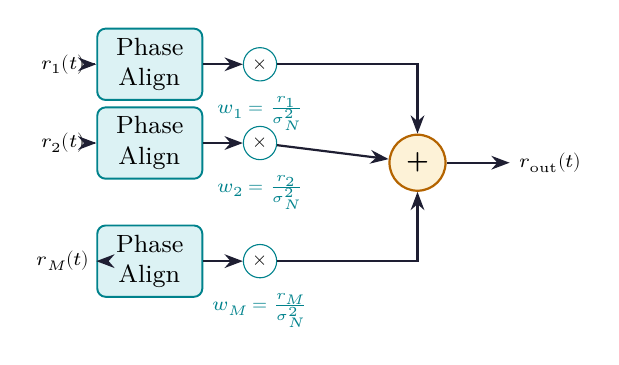
\begin{tikzpicture}[node distance=0.6cm and 1.0cm, every node/.style={font=\scriptsize}]
  % Inputs
  \node (r1) at (0, 1.5) {$r_1(t)$};
  \node (r2) at (0, 0.5) {$r_2(t)$};
  \node (rM) at (0, -1.0) {$r_M(t)$};
  \node at (0, -0.25) {\vdots};

  % Weight multipliers
  \node[circle, draw=myteal, inner sep=2pt] (m1) at (2.5, 1.5) {$\times$};
  \node[circle, draw=myteal, inner sep=2pt] (m2) at (2.5, 0.5) {$\times$};
  \node[circle, draw=myteal, inner sep=2pt] (mM) at (2.5, -1.0) {$\times$};

  % Weight labels below multipliers
  \node[below=2pt of m1, color=myteal] {$w_1 = \frac{r_1}{\sigma_N^2}$};
  \node[below=2pt of m2, color=myteal] {$w_2 = \frac{r_2}{\sigma_N^2}$};
  \node[below=2pt of mM, color=myteal] {$w_M = \frac{r_M}{\sigma_N^2}$};

  % Phase adjusters (in-between)
  \node[block, text width=1.1cm, minimum height=0.6cm] (p1) at (1.1, 1.5) {Phase\\Align};
  \node[block, text width=1.1cm, minimum height=0.6cm] (p2) at (1.1, 0.5) {Phase\\Align};
  \node[block, text width=1.1cm, minimum height=0.6cm] (pM) at (1.1, -1.0) {Phase\\Align};

  % Summation
  \node[sumjunc] (sum) at (4.5, 0.25) {\textbf{+}};
  \node[right=0.8cm of sum] (out) {$r_{\text{out}}(t)$};

  % Connections
  \draw[arrow] (r1) -- (p1); \draw[arrow] (p1) -- (m1);
  \draw[arrow] (r2) -- (p2); \draw[arrow] (p2) -- (m2);
  \draw[arrow] (rM) -- (pM); \draw[arrow] (pM) -- (mM);

  \draw[arrow] (m1) -| (sum);
  \draw[arrow] (m2) -- (sum);
  \draw[arrow] (mM) -| (sum);
  
  \draw[arrow] (sum) -- (out);
\end{tikzpicture}
\end{tcolorbox}

% ===============================================================================
\section{RAKE Receiver}
% ===============================================================================

In wideband CDMA systems, the signal bandwidth is larger than the coherence bandwidth of the channel, making the channel frequency-selective. This time dispersion resolved as distinct multipath components is exploited by the RAKE receiver.

\begin{tcolorbox}[defbox]
\textbf{RAKE Receiver:} A receiver designed for spread-spectrum CDMA systems that uses multiple parallel correlators called \textbf{fingers} to independently track, delay-align, and combine individual multipath components, turning time dispersion into a source of diversity.
\end{tcolorbox}

\subsection{Working Principle}
\begin{itemize}[leftmargin=*, itemsep=3.0pt]
  \item \textbf{Resolution:} The chip duration ($T_c$) of a CDMA code is very short. If the difference in propagation delay between two paths is greater than $T_c$, the receiver can resolve them as independent paths.
  \item \textbf{Fingers:} The RAKE receiver allocates one "finger" to each resolved multipath component. Each finger correlates the received signal with a delayed version of the spreading code $c(t - \tau_i)$ corresponding to that path's excess delay $\tau_i$.
  \item \textbf{Combining:} The outputs of all fingers are co-phased and combined using Maximal Ratio Combining (MRC).
\end{itemize}

\begin{tcolorbox}[tikzbox, title={RAKE Receiver Finger Structure}]
\centering
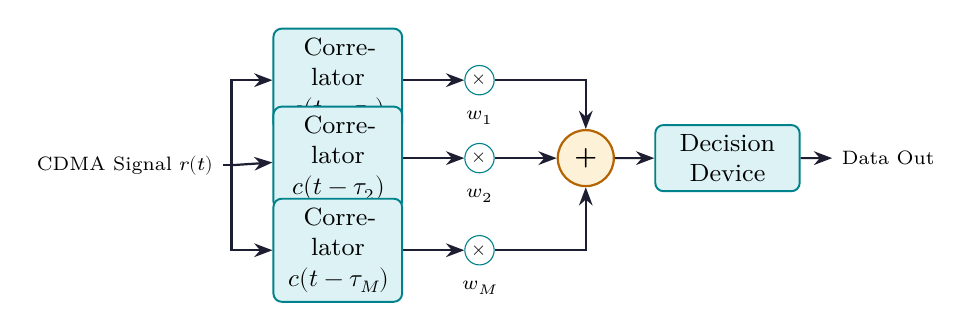
\begin{tikzpicture}[scale=0.9, every node/.style={font=\scriptsize}]
  % Input
  \node (in) at (-1, 0) {CDMA Signal $r(t)$};

  % Split into fingers
  \node[block, text width=1.4cm, minimum height=0.7cm] (cor1) at (2, 1.2) {Correlator\\$c(t-\tau_1)$};
  \node[block, text width=1.4cm, minimum height=0.7cm] (cor2) at (2, 0.1) {Correlator\\$c(t-\tau_2)$};
  \node[block, text width=1.4cm, minimum height=0.7cm] (corM) at (2, -1.2) {Correlator\\$c(t-\tau_M)$};

  % Multipliers
  \node[circle, draw=myteal, inner sep=1.5pt] (m1) at (4.0, 1.2) {$\times$};
  \node[circle, draw=myteal, inner sep=1.5pt] (m2) at (4.0, 0.1) {$\times$};
  \node[circle, draw=myteal, inner sep=1.5pt] (mM) at (4.0, -1.2) {$\times$};

  \node[below=2pt of m1] {$w_1$};
  \node[below=2pt of m2] {$w_2$};
  \node[below=2pt of mM] {$w_M$};

  % Summation
  \node[sumjunc] (sum) at (5.5, 0.1) {\textbf{+}};
  \node[block, right=0.5cm of sum, text width=1.6cm, minimum height=0.7cm] (det) {Decision\\Device};
  \node[right=0.4cm of det] (out) {Data Out};

  % Connect lines
  \draw[line] (in) -- (0.5, 0);
  \draw[arrow] (0.5, 0) |- (cor1);
  \draw[arrow] (0.5, 0) -- (cor2);
  \draw[arrow] (0.5, 0) |- (corM);

  \draw[arrow] (cor1) -- (m1);
  \draw[arrow] (cor2) -- (m2);
  \draw[arrow] (corM) -- (mM);

  \draw[arrow] (m1) -| (sum);
  \draw[arrow] (m2) -- (sum);
  \draw[arrow] (mM) -| (sum);

  \draw[arrow] (sum) -- (det);
  \draw[arrow] (det) -- (out);
\end{tikzpicture}
\end{tcolorbox}

% ===============================================================================
\section{Channel Equalization}
% ===============================================================================

Equalizers combat Inter-Symbol Interference (ISI) caused by time-dispersive fading channels by modeling the inverse of the channel's transfer function.

\subsection{Linear Equalizers}
Linear equalizers process the received signal using a linear transversal filter (Tapped Delay Line):
\begin{enumerate}[label=\textbf{\arabic*.}, leftmargin=*, itemsep=3.5pt]
  \item \textbf{Zero-Forcing Equalizer (ZFE):} Forces the equalizer output to have zero ISI at the decision points. Its frequency response is the exact inverse of the channel response:
    \begin{equation}
      H_{\text{eq}}(f) = \frac{1}{H(f)}
    \end{equation}
    \textbf{Limitation:} In spectral nulls (frequencies where the channel gain $H(f)$ is very small), ZFE heavily amplifies the noise.
  \item \textbf{Minimum Mean Square Error (MMSE) Equalizer:} Minimizes the mean square error between the actual transmitted symbol and the equalizer output, providing a balance between ISI mitigation and noise amplification:
    \begin{equation}
      H_{\text{eq}}(f) = \frac{H^*(f)}{|H(f)|^2 + \frac{N_0}{E_s}}
    \end{equation}
\end{enumerate}

\subsection{Adaptive Equalizers}
Since mobile channels are time-varying, the equalizer coefficients must adapt dynamically.
\begin{itemize}[leftmargin=*, itemsep=3.0pt]
  \item \textbf{LMS (Least Mean Squares) Algorithm:} A gradient-descent optimization algorithm that adjusts coefficients iteratively to minimize the mean square error. It is simple to implement but has a slow convergence rate.
  \item \textbf{RLS (Recursive Least Squares) Algorithm:} A more complex algorithm that utilizes least-squares estimation to update weights. It converges much faster than LMS but has significantly higher computational complexity.
\end{itemize}

\subsection{Non-linear Equalizers (Decision Feedback Equalizer - DFE)}
When the channel has severe spectral nulls, linear equalizers perform poorly due to noise amplification. Non-linear equalizers solve this:
\begin{itemize}[leftmargin=*, itemsep=3.0pt]
  \item \textbf{DFE Structure:} Consists of a \textbf{Feedforward Filter} (similar to a linear equalizer) and a \textbf{Feedback Filter}.
  \item \textbf{Feedback Mechanism:} The feedback filter takes previously decided symbols, reconstructs the resulting ISI, and subtracts it from the current input before the decision device. Because the subtracted ISI is based on clean decided symbols, it introduces no noise amplification.
\end{itemize}

% ===============================================================================
\section{Transmit Diversity and the Alamouti Scheme}
% ===============================================================================

Transmit diversity shifts the complexity of multiple antennas from the mobile terminal (downlink receiver) to the base station (downlink transmitter).

\subsection{The Alamouti Scheme (2x1 MIMO)}
The Alamouti scheme is a simple and elegant space-time block coding (STBC) method that achieves a diversity order of 2 using two transmit antennas ($Tx_0, Tx_1$) and one receive antenna ($Rx$).

\begin{tcolorbox}[tikzbox, title={Alamouti 2x1 Transmit Diversity Configuration}]
\centering
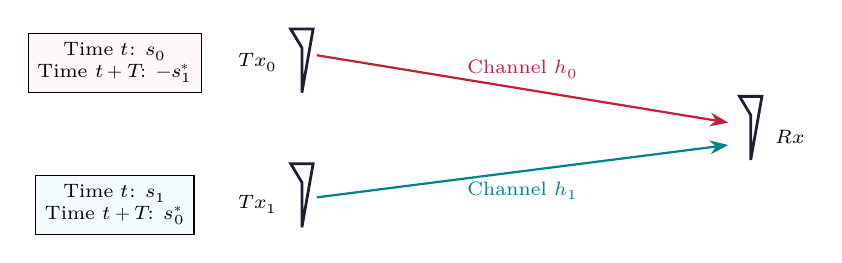
\begin{tikzpicture}[scale=0.95, every node/.style={font=\scriptsize}]
  % Transmit Antennas
  \draw[line, line width=1pt] (0, 1.2) -- (0, 1.8) -- (-0.15, 2.05) -- (0.15, 2.05) -- cycle;
  \node[left] at (-0.2, 1.6) {$Tx_0$};
  
  \draw[line, line width=1pt] (0, -0.6) -- (0, 0.0) -- (-0.15, 0.25) -- (0.15, 0.25) -- cycle;
  \node[left] at (-0.2, -0.3) {$Tx_1$};

  % Receiver Antenna
  \draw[line, line width=1pt] (6, 0.3) -- (6, 0.9) -- (5.85, 1.15) -- (6.15, 1.15) -- cycle;
  \node[right] at (6.2, 0.6) {$Rx$};

  % Channel lines
  \draw[arrow, color=myred] (0.2, 1.7) -- (5.7, 0.8) node[midway, above] {Channel $h_0$};
  \draw[arrow, color=myteal] (0.2, -0.2) -- (5.7, 0.5) node[midway, below] {Channel $h_1$};

  % Space-Time mapping tables
  \node[draw, fill=hdrred!30, align=center] at (-2.5, 1.6) {Time $t$: $s_0$\\Time $t+T$: $-s_1^*$};
  \node[draw, fill=hdrteal!30, align=center] at (-2.5, -0.3) {Time $t$: $s_1$\\Time $t+T$: $s_0^*$};
\end{tikzpicture}
\end{tcolorbox}

\subsection{Space-Time Block Coding Matrix and Derivation}
The transmit scheme maps two symbols $s_0$ and $s_1$ over two symbol periods ($t$ and $t+T$):
\par\noindent
{\renewcommand{\arraystretch}{1.65}%
\begin{tabularx}{\linewidth}{|B{3.2cm}|Y|Y|}\hline
\textbf{Antenna / Time} & \textbf{Time $t$} & \textbf{Time $t+T$} \\
\hline
\textbf{Antenna $Tx_0$} & $s_0$ & $-s_1^*$ \\[4pt]
\hline
\textbf{Antenna $Tx_1$} & $s_1$ & $s_0^*$ \\[4pt]
\hline
\end{tabularx}
}

Let $h_0$ and $h_1$ be the complex channel gains from $Tx_0$ and $Tx_1$ to the receive antenna, assumed constant over both symbol periods. The received signals $r_0$ and $r_1$ are:
\begin{equation}
  r_0 = r(t) = h_0 s_0 + h_1 s_1 + n_0
\end{equation}
\begin{equation}
  r_1 = r(t+T) = -h_0 s_1^* + h_1 s_0^* + n_1
\end{equation}
Where $n_0, n_1$ are AWGN noise terms. Taking the conjugate of $r_1$:
\begin{equation}
  r_1^* = -h_0^* s_1 + h_1^* s_0 + n_1^*
\end{equation}
We can write this in matrix form:
\begin{equation}
  \begin{bmatrix} r_0 \\ r_1^* \end{bmatrix} = \begin{bmatrix} h_0 & h_1 \\ h_1^* & -h_0^* \end{bmatrix} \begin{bmatrix} s_0 \\ s_1 \end{bmatrix} + \begin{bmatrix} n_0 \\ n_1^* \end{bmatrix}
\end{equation}
Let $\mathbf{H}_{\text{eff}} = \begin{bmatrix} h_0 & h_1 \\ h_1^* & -h_0^* \end{bmatrix}$ be the effective channel matrix. The columns of $\mathbf{H}_{\text{eff}}$ are orthogonal:
\begin{equation}
  \mathbf{H}_{\text{eff}}^H \mathbf{H}_{\text{eff}} = \left( |h_0|^2 + |h_1|^2 \right) \mathbf{I}_2
\end{equation}
The receiver decodes the symbols by multiplying the received vector by $\mathbf{H}_{\text{eff}}^H$:
\begin{equation}
  \begin{bmatrix} \tilde{s}_0 \\ \tilde{s}_1 \end{bmatrix} = \mathbf{H}_{\text{eff}}^H \begin{bmatrix} r_0 \\ r_1^* \end{bmatrix} = \begin{bmatrix} h_0^* r_0 + h_1 r_1^* \\ h_1^* r_0 - h_0 r_1^* \end{bmatrix}
\end{equation}
Expanding for symbol $s_0$:
\begin{equation}
  \tilde{s}_0 = \left( |h_0|^2 + |h_1|^2 \right) s_0 + h_0^* n_0 + h_1 n_1^*
\end{equation}
This yields an exact diversity order of 2, equivalent to 1x2 MRC at the receiver, but implemented at the transmitter.

% ===============================================================================
% MANDATORY QUICK REVISION PAGE
% ===============================================================================
\newpage
\begin{center}
  {\large\bfseries\color{myred} Quick Revision --- Module V}\\[3pt]
  {\small\color{mydark} Receiver Structure and Diversity Techniques $|$ PE-EC701C}
\end{center}
\noindent{\color{myred}\rule{\linewidth}{1.2pt}}
\vspace{4pt}

\begin{tcolorbox}[formulabox, title={\textbf{Key Formulas at a Glance}}]
\renewcommand{\arraystretch}{1.3}
\begin{tabularx}{\linewidth}{B{5.5cm} X}Selection Combining (SC) SNR & $\gamma_{\text{out}} = \max(\gamma_1, \gamma_2, \dots, \gamma_M)$ \\
Maximal Ratio Combining (MRC) SNR & $\gamma_{\text{out}} = \sum_{i=1}^{M} \gamma_i$ \\
Linear Equalizer Output & $\hat{d}_k = \sum c_n y_{k-n}$ \\
Zero-Forcing Filter Relation & $H_{\text{eq}}(f) = \frac{1}{H(f)}$ \\
MMSE Filter Relation & $H_{\text{eq}}(f) = \frac{H^*(f)}{|H(f)|^2 + N_0/E_s}$ \\
Alamouti Matrix Orthogonality & $\mathbf{H}_{\text{eff}}^H \mathbf{H}_{\text{eff}} = \left( |h_0|^2 + |h_1|^2 \right) \mathbf{I}_2$ \\
Alamouti Decoded Symbol & $\tilde{s}_0 = h_0^* r_0 + h_1 r_1^*$
\end{tabularx}
\end{tcolorbox}

\begin{tcolorbox}[defbox, title={\textbf{One-Line Definitions}}]
\begin{itemize}[leftmargin=*, itemsep=2.5pt, topsep=0pt]
  \item \textbf{Selection Combining:} Diversity method selecting the single branch with the highest instantaneous SNR.
  \item \textbf{Maximal Ratio Combining:} Optimal combining method that co-phases and weights branches by their signal-to-noise ratio.
  \item \textbf{RAKE Receiver:} A CDMA receiver utilizing multiple correlator fingers to combine resolved multipath components.
  \item \textbf{Zero-Forcing Equalizer:} A linear equalizer that inverts the channel response, completely eliminating ISI at the cost of noise amplification.
  \item \textbf{DFE:} Decision Feedback Equalizer, a non-linear equalizer that subtracts the ISI of previously decided symbols.
  \item \textbf{Alamouti Scheme:} A 2x1 transmit diversity scheme mapping symbols over space and time using orthogonal block codes.
  \item \textbf{Space-Time Block Code:} Mapping data streams over multiple antennas and time slots to achieve transmit diversity.
\end{itemize}
\end{tcolorbox}

\begin{tcolorbox}[exambox, title={\textbf{Frequently Asked / Viva Questions}}]
\begin{enumerate}[topsep=0pt, label=\textbf{Q\arabic*.}, itemsep=5pt]
  \item \Q{Compare Selection Combining (SC) and Maximal Ratio Combining (MRC).}
    SC selects only the single branch with the highest instantaneous SNR. MRC co-phases and sums all branches weighted by their SNRs, maximizing performance by summing all signal energies.
  \item \Q{What is a RAKE receiver? Why is it named after a rake?}
    It is a CDMA receiver that resolves multipath components using parallel correlator fingers. It is named after a garden rake because it "rakes" together scattered multipath energies into a single coherent signal.
  \item \Q{Explain the noise amplification problem in Zero-Forcing Equalizers.}
    ZFE completely inverts the channel frequency response ($H_{\text{eq}} = 1/H(f)$). In deep channel fades (spectral nulls), $H(f) \to 0$, causing $H_{\text{eq}}$ to become extremely large, amplifying the background noise.
  \item \Q{Why does a Decision Feedback Equalizer (DFE) avoid noise amplification?}
    It uses a feedback filter to subtract the ISI caused by previously detected symbols. Because the feedback signal is derived from clean decided symbols rather than the noisy received signal, it introduces no noise.
  \item \Q{Derive the effective channel matrix and prove orthogonality in the Alamouti scheme.}
    $\mathbf{H}_{\text{eff}} = \begin{bmatrix} h_0 & h_1 \\ h_1^* & -h_0^* \end{bmatrix}$. Multiplying by its conjugate transpose: $\mathbf{H}_{\text{eff}}^H \mathbf{H}_{\text{eff}} = \begin{bmatrix} h_0^* & h_1 \\ h_1^* & -h_0 \end{bmatrix} \begin{bmatrix} h_0 & h_1 \\ h_1^* & -h_0^* \end{bmatrix} = \begin{bmatrix} |h_0|^2+|h_1|^2 & 0 \\ 0 & |h_0|^2+|h_1|^2 \end{bmatrix} = (|h_0|^2+|h_1|^2)\mathbf{I}_2$.
  \item \Q{State the antenna spacing requirements for space diversity.}
    To ensure uncorrelated fading, the spacing should be at least $0.5\lambda$ at the mobile terminal (due to rich local scattering) and $10\lambda$ to $20\lambda$ at the base station (due to high elevation and narrow angle of arrival).
  \item \Q{What are the advantages of polarization diversity over spatial diversity?}
    Polarization diversity uses orthogonal states (e.g. $\pm 45^\circ$) on a single physical antenna structure. It requires no physical spacing between antennas, saving base station tower space.
  \item \Q{What is the difference between LMS and RLS adaptive algorithms?}
    LMS uses a gradient-descent approach; it is simple but converges slowly. RLS uses recursive least-squares; it has high computational complexity but converges much faster.
  \item \Q{Explain the physical meaning of "co-phasing" in diversity combining.}
    Fading introduces independent phase shifts on each branch. Before summing the signals, the receiver must align their phases to prevent destructive interference (phase cancellation).
  \item \Q{Under what condition can a RAKE receiver resolve multipath components?}
    The delay difference between the multipath components must exceed the CDMA chip duration ($|\tau_1 - \tau_2| > T_c$). Otherwise, the paths cannot be separated.
  \item \Q{What is Equal Gain Combining (EGC)?}
    A combining method where branch signals are co-phased and summed with equal weights ($w_i=1$). It avoids the complex circuitry required to estimate signal amplitudes.
  \item \Q{Why is transmit diversity preferred over receive diversity in downlink design?}
    Adding multiple antennas to a mobile terminal increases its size, cost, and power consumption. Transmit diversity achieves similar performance gains by putting the multiple antennas on the base station.
\end{enumerate}
\tcbset{colbacktitle=myteal, coltitle=white}
\end{tcolorbox}

\begin{tcolorbox}[tikzbox, title={Comparison of Diversity Combining Methods}]
\renewcommand{\arraystretch}{1.4}
\par\noindent
{\renewcommand{\arraystretch}{1.55}%
\begin{tabularx}{\linewidth}{|B{3.0cm}|Y|Y|Y|}\hline
\textbf{Parameter} & \textbf{Selection Combining} & \textbf{Equal Gain} & \textbf{Maximal Ratio} \\
\hline
\textbf{Logic} & Selects highest SNR branch. & Co-phases and sums equally. & Co-phases and weights by SNR. \\[4pt]
\hline
\textbf{Complexity} & Low (no phase tracking needed). & Medium (requires co-phasing only). & High (requires phase and amplitude tracking). \\[4pt]
\hline
\textbf{Performance} & Lowest SNR gain. & Close to MRC ($\approx 1$ dB loss). & Optimal SNR gain. \\
\hline
\end{tabularx}
}
\tcbset{colbacktitle=myteal, coltitle=white}
\end{tcolorbox}


% -- Module 6 -----------------------------------------------------------------
\modulestart{6}{Multiple-Input Multiple-Output (MIMO) Systems}

\section{Multiple-Input Multiple-Output (MIMO) Systems}
% ===============================================================================

MIMO systems employ multiple antennas at both the transmitter and receiver to improve link reliability and throughput without requiring extra bandwidth or transmit power.

\begin{tcolorbox}[defbox]
\textbf{MIMO System:} A wireless technology utilizing $N_T$ transmit antennas and $N_R$ receive antennas to establish a multi-antenna channel. The received signal vector $\mathbf{y}$ is modeled as:
\begin{equation}
  \mathbf{y} = \mathbf{H} \mathbf{x} + \mathbf{n}
\end{equation}
Where $\mathbf{x}$ is the $N_T \times 1$ transmitted vector, $\mathbf{y}$ is the $N_R \times 1$ received vector, $\mathbf{n}$ is the $N_R \times 1$ noise vector, and $\mathbf{H}$ is the $N_R \times N_T$ channel matrix containing complex gains $h_{ij}$ between transmit antenna $j$ and receive antenna $i$.
\end{tcolorbox}

\begin{tcolorbox}[tikzbox, title={MIMO System Model and Channel Matrix}]
\centering
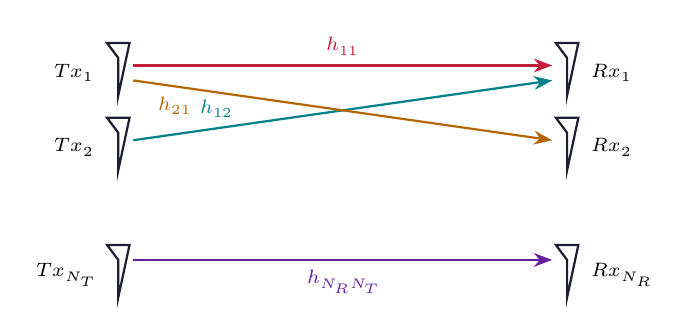
\begin{tikzpicture}[scale=0.95, every node/.style={font=\scriptsize}]
  % Tx Antennas
  \draw[line] (-2, 1.5) -- (-2, 2.0) -- (-2.15, 2.2) -- (-1.85, 2.2) -- cycle;
  \node[left] at (-2.2, 1.8) {$Tx_1$};
  
  \draw[line] (-2, 0.5) -- (-2, 1.0) -- (-2.15, 1.2) -- (-1.85, 1.2) -- cycle;
  \node[left] at (-2.2, 0.8) {$Tx_2$};
  
  \node at (-2, -0.1) {\vdots};
  
  \draw[line] (-2, -1.2) -- (-2, -0.7) -- (-2.15, -0.5) -- (-1.85, -0.5) -- cycle;
  \node[left] at (-2.2, -0.9) {$Tx_{N_T}$};

  % Rx Antennas
  \draw[line] (4, 1.5) -- (4, 2.0) -- (3.85, 2.2) -- (4.15, 2.2) -- cycle;
  \node[right] at (4.2, 1.8) {$Rx_1$};
  
  \draw[line] (4, 0.5) -- (4, 1.0) -- (3.85, 1.2) -- (4.15, 1.2) -- cycle;
  \node[right] at (4.2, 0.8) {$Rx_2$};
  
  \node at (4, -0.1) {\vdots};
  
  \draw[line] (4, -1.2) -- (4, -0.7) -- (3.85, -0.5) -- (4.15, -0.5) -- cycle;
  \node[right] at (4.2, -0.9) {$Rx_{N_R}$};

  % Channel matrix connections (sample)
  \draw[arrow, color=myred] (-1.8, 1.9) -- (3.8, 1.9) node[midway, above] {$h_{11}$};
  \draw[arrow, color=myteal] (-1.8, 0.9) -- (3.8, 1.7) node[pos=0.2, above] {$h_{12}$};
  \draw[arrow, color=myamber] (-1.8, 1.7) -- (3.8, 0.9) node[pos=0.1, below] {$h_{21}$};
  \draw[arrow, color=mypurple] (-1.8, -0.7) -- (3.8, -0.7) node[midway, below] {$h_{N_R N_T}$};
\end{tikzpicture}
\end{tcolorbox}

\subsection{Spatial Multiplexing vs. Spatial Diversity}
MIMO antennas can be used in two distinct modes to serve different system goals:
\par\noindent
{\renewcommand{\arraystretch}{1.65}%
\begin{tabularx}{\linewidth}{|B{3.2cm}|Y|Y|}\hline
\textbf{Feature} & \textbf{Spatial Multiplexing} & \textbf{Spatial Diversity} \\
\hline
\textbf{Primary Goal} & Maximizes data rate (throughput). & Maximizes link reliability (reduces BER). \\[4pt]
\hline
\textbf{Transmission} & Transmits different data streams from each antenna simultaneously. & Transmits the same or coded data streams from multiple antennas. \\[4pt]
\hline
\textbf{Capacity Scaling} & Scales linearly with $\min(N_T, N_R)$. & No rate increase, but stabilizes signal SNR. \\[4pt]
\hline
\textbf{Key Schemes} & V-BLAST (Bell Labs Layered Space-Time). & Alamouti code, Space-Time Block Coding (STBC). \\[4pt]
\hline
\textbf{Channel Condition} & Requires high SNR and rich scattering. & Effective in poor SNR and deep fades. \\[4pt]
\hline
\end{tabularx}
}

\subsection{MIMO Channel Capacity}
If the channel state information (CSI) is known at the receiver only, and transmit power is distributed equally among all transmit antennas, the capacity is:
\begin{equation}
  C = B \log_2 \det \left( \mathbf{I}_{N_R} + \frac{\text{SNR}}{N_T} \mathbf{H} \mathbf{H}^H \right)
\end{equation}
Under independent and identically distributed (i.i.d.) Rayleigh fading, as $N_T, N_R \to \infty$, capacity scales as:
\begin{equation}
  C \approx \min(N_T, N_R) \cdot B \log_2(1 + \text{SNR})
\end{equation}

\subsection{Diversity-Multiplexing Trade-off (DMT)}
In MIMO systems, we cannot maximize both multiplexing gain and diversity gain simultaneously.
\begin{itemize}[leftmargin=*, itemsep=3pt]
  \item \textbf{Multiplexing Gain ($r$):} Measures how fast the transmission rate scales with SNR.
  \item \textbf{Diversity Gain ($d$):} Measures how fast the bit error rate (BER) decays with SNR ($P_e \propto \text{SNR}^{-d}$).
  \item \textbf{Trade-off Relation:} For a flat-fading i.i.d. MIMO channel of size $N_T \times N_R$, the optimal trade-off is a piecewise linear function. The maximum diversity gain at multiplexing gain $r$ (for integer $r$) is:
    \begin{equation}
      d^*(r) = (N_T - r)(N_R - r)
    \end{equation}
    For $r=0$ (pure diversity), $d^* = N_T N_R$. For $r=\min(N_T, N_R)$ (pure multiplexing), $d^* = 0$.
\end{itemize}

% ===============================================================================
\section{Cellular System Examples}
% ===============================================================================

\subsection{GSM (Global System for Mobile Communications)}
GSM is the definitive 2G digital cellular standard, operating primarily in the 900 MHz and 1800 MHz bands.

\begin{tcolorbox}[defbox]
\textbf{GSM Architecture:} Comprises three main subsystems:
\begin{itemize}[leftmargin=*, itemsep=2.5pt, topsep=2pt]
  \item \textbf{Mobile Station (MS):} The user handset containing the Subscriber Identity Module (SIM).
  \item \textbf{Base Station Subsystem (BSS):} Consists of the Base Transceiver Station (BTS - antennas and transceivers) and the Base Station Controller (BSC - handles radio resource allocation and handovers).
  \item \textbf{Network and Switching Subsystem (NSS):} The core network, centered on the Mobile Switching Center (MSC - routes calls) and databases: HLR (Home Location Register), VLR (Visitor Location Register), AuC (Authentication Center), and EIR (Equipment Identity Register).
\end{itemize}
\end{tcolorbox}

\begin{tcolorbox}[tikzbox, title={GSM System Architecture Block Diagram}]
\centering
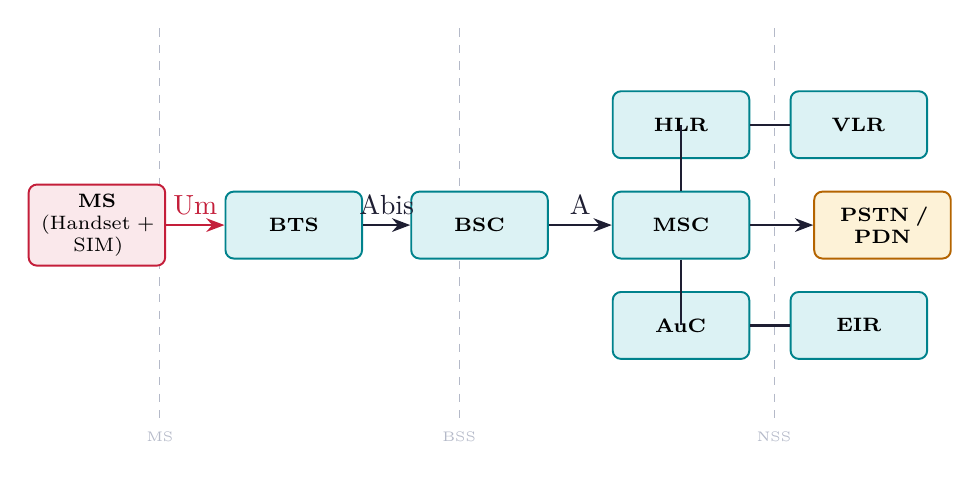
\begin{tikzpicture}[node distance=0.4cm and 0.55cm,
  sblock/.style={rectangle, draw=myteal, fill=hdrteal, text width=1.5cm,
    align=center, minimum height=0.85cm, font=\scriptsize,
    rounded corners=3pt, line width=0.7pt}]

  % Subsystems demarcation
  \draw[dashed, color=mgframe] (-2.2, 2.5) -- (-2.2, -2.5) node[below, font=\tiny] {MS};
  \draw[dashed, color=mgframe] (1.6, 2.5) -- (1.6, -2.5) node[below, font=\tiny] {BSS};
  \draw[dashed, color=mgframe] (5.6, 2.5) -- (5.6, -2.5) node[below, font=\tiny] {NSS};

  % MS Nodes
  \node[sblock, draw=myred, fill=hdrred] (ms) at (-3, 0) {\textbf{MS}\\(Handset +\\SIM)};

  % BSS Nodes
  \node[sblock] (bts) at (-0.5, 0) {\textbf{BTS}};
  \node[sblock, right=0.6cm of bts] (bsc) {\textbf{BSC}};

  % NSS Nodes
  \node[sblock, right=0.8cm of bsc] (msc) {\textbf{MSC}};
  \node[sblock, above=0.4cm of msc] (hlr) {\textbf{HLR}};
  \node[sblock, right=0.5cm of hlr] (vlr) {\textbf{VLR}};
  \node[sblock, below=0.4cm of msc] (auc) {\textbf{AuC}};
  \node[sblock, right=0.5cm of auc] (eir) {\textbf{EIR}};

  % External Network
  \node[sblock, right=0.8cm of msc, draw=myamber, fill=hdramber] (pstn) {\textbf{PSTN /}\\ \textbf{PDN}};

  % Connections
  \draw[arrow, redarrow] (ms) -- (bts) node[midway, above] {Um};
  \draw[arrow] (bts) -- (bsc) node[midway, above] {Abis};
  \draw[arrow] (bsc) -- (msc) node[midway, above] {A};
  \draw[arrow] (msc) -- (pstn);
  
  \draw[line] (msc) |- (hlr);
  \draw[line] (msc) |- (auc);
  \draw[line] (hlr) -- (vlr);
  \draw[line] (auc) -- (eir);
\end{tikzpicture}
\end{tcolorbox}

\subsubsection{GSM Channels}
GSM uses a combination of FDMA and TDMA. Each carrier is 200 kHz wide, divided into 8 time slots (users). Channels are divided into:
\begin{itemize}[leftmargin=*, itemsep=3.0pt]
  \item \textbf{Physical Channel:} A specific RF carrier frequency and time slot number.
  \item \textbf{Logical Channels:} Mapped onto physical channels to carry specific types of data.
    \begin{itemize}[leftmargin=*, itemsep=2.5pt, topsep=2pt]
      \item \textbf{Traffic Channels (TCH):} Carry digitized speech or user data.
      \item \textbf{Control Channels (CCH):} Carry signaling and control information:
        \begin{itemize}[leftmargin=*, itemsep=2pt, topsep=2pt]
          \item \textit{Broadcast Channels (BCH):} Broadcast system parameters (BCCH) and frequency correction (FCCH/SCH).
          \item \textit{Common Control Channels (CCCH):} Handle paging (PCH) and random access (RACH) to set up calls.
          \item \textit{Dedicated Control Channels (DCCH):} Handle registration and SMS.
        \end{itemize}
    \end{itemize}
\end{itemize}

\subsection{GPRS and EDGE}
\begin{itemize}[leftmargin=*, itemsep=3pt]
  \item \textbf{GPRS (General Packet Radio Service - 2.5G):} Introduces packet switching to the circuit-switched GSM core. Adds two new nodes: GGSN (Gateway GPRS Support Node) and SGSN (Serving GPRS Support Node). Supports data rates up to 115 kbps using GMSK modulation.
  \item \textbf{EDGE (Enhanced Data Rates for GSM Evolution - 2.75G):} Updates the modulation scheme from GMSK to \textbf{8-PSK} (Phase Shift Keying). Because 8-PSK maps 3 bits per symbol (instead of 1 bit in GMSK), EDGE triples the data rate of GSM/GPRS, achieving throughputs up to 384 kbps within the same 200 kHz channels.
\end{itemize}

\subsection{IS-95 (cdmaOne)}
IS-95 is the first CDMA-based 2G standard, operating in 1.25 MHz channels.
\begin{itemize}[leftmargin=*, itemsep=3pt]
  \item \textbf{Forward Link Channels (Base Station to Mobile):} Modulated using Walsh codes (length 64) for user separation and a pilot PN sequence. Channels include Pilot, Sync, Paging, and Forward Traffic Channels.
  \item \textbf{Reverse Link Channels (Mobile to Base Station):} Separated using unique offsets of a long PN code. Channels include Access and Reverse Traffic Channels.
\end{itemize}

\subsection{3G Standards: WCDMA and CDMA2000}
\begin{itemize}[leftmargin=*, itemsep=3pt]
  \item \textbf{WCDMA (Wideband CDMA / UMTS):} The dominant 3G standard. Operates in 5 MHz channels (chip rate of 3.84 Mcps). Supports asynchronous base stations and coherent detection on the uplink using pilot symbols.
  \item \textbf{CDMA2000:} A 3G standard evolution of IS-95. Uses a chip rate of 1.2288 Mcps (1xRTT) and is backward compatible with IS-95 hardware.
\end{itemize}

% ===============================================================================
% MANDATORY QUICK REVISION PAGE
% ===============================================================================
\newpage
\begin{center}
  {\large\bfseries\color{myred} Quick Revision --- Module VI}\\[3pt]
  {\small\color{mydark} MIMO and Cellular System Examples $|$ PE-EC701C}
\end{center}
\noindent{\color{myred}\rule{\linewidth}{1.2pt}}
\vspace{4pt}

\begin{tcolorbox}[formulabox, title={\textbf{Key Formulas at a Glance}}]
\renewcommand{\arraystretch}{1.3}
\begin{tabularx}{\linewidth}{B{5.5cm} X}MIMO System Equation & $\mathbf{y} = \mathbf{H} \mathbf{x} + \mathbf{n}$ \\
MIMO Capacity (No CSIT) & $C = B \log_2 \det \left( \mathbf{I}_{N_R} + \frac{\text{SNR}}{N_T} \mathbf{H} \mathbf{H}^H \right)$ \\
MIMO Asymptotic Capacity & $C \approx \min(N_T, N_R) \cdot B \log_2(1 + \text{SNR})$ \\
Optimal DMT Trade-off & $d^*(r) = (N_T - r)(N_R - r)$ \\
GSM Carrier Bandwidth & $B = 200 \text{ kHz}$ \quad (divided into 8 time slots) \\
EDGE Modulation Update & GMSK (1 bit/symbol) $\to$ 8-PSK (3 bits/symbol) \\
IS-95 Channel Bandwidth & $B = 1.25 \text{ MHz}$ \quad (chip rate = 1.2288 Mcps) \\
WCDMA Channel Bandwidth & $B = 5.0 \text{ MHz}$ \quad (chip rate = 3.84 Mcps)
\end{tabularx}
\end{tcolorbox}

\begin{tcolorbox}[defbox, title={\textbf{One-Line Definitions}}]
\begin{itemize}[leftmargin=*, itemsep=2.5pt, topsep=0pt]
  \item \textbf{MIMO:} Using multiple antennas at transmitter and receiver to boost data rate and reliability.
  \item \textbf{Spatial Multiplexing:} Transmitting independent data streams from multiple antennas to increase throughput.
  \item \textbf{Spatial Diversity:} Sending coded redundant signals from multiple antennas to increase link reliability.
  \item \textbf{GSM BSC:} Node in BSS responsible for radio channel allocation and mobile handover management.
  \item \textbf{HLR:} Home Location Register, the central database storing subscription details and location info for home users.
  \item \textbf{GPRS SGSN:} Node responsible for packet routing, mobility management, and authentication of packet data.
  \item \textbf{8-PSK:} Modulation scheme used in EDGE mapping 3 bits per symbol, tripling GPRS data rates.
\end{itemize}
\end{tcolorbox}

\begin{tcolorbox}[exambox, title={\textbf{Frequently Asked / Viva Questions}}]
\begin{enumerate}[topsep=0pt, label=\textbf{Q\arabic*.}, itemsep=5pt]
  \item \Q{Compare spatial multiplexing and spatial diversity in MIMO systems.}
    Spatial multiplexing transmits different data streams from each antenna, maximizing data rate ($C \propto \min(N_T, N_R)$). Spatial diversity transmits redundant coded versions of the same signal, maximizing link reliability.
  \item \Q{Explain the diversity-multiplexing trade-off (DMT).}
    A MIMO channel can provide multiplexing gain $r$ and diversity gain $d$ simultaneously, but they are inversely related: $d^*(r) = (N_T - r)(N_R - r)$. You cannot maximize both at the same time.
  \item \Q{Draw and explain the GSM BSS architecture.}
    The Base Station Subsystem (BSS) contains the Base Transceiver Station (BTS) which handles the RF transmission and antennas, and the Base Station Controller (BSC) which manages handover decisions and radio channel allocations.
  \item \Q{Define the roles of HLR and VLR in GSM.}
    HLR is the master database containing subscription profiles and current location coordinates of all home subscribers. VLR is a local database containing profiles of roaming users currently inside that MSC's area.
  \item \Q{How does EDGE achieve higher data rates than GPRS within the same channel bandwidth?}
    EDGE replaces GMSK modulation (1 bit per symbol) with 8-PSK modulation (3 bits per symbol). By mapping 3 bits per symbol, it triples the data rate to 384 kbps without widening the 200 kHz channel.
  \item \Q{What are the functions of the SGSN and GGSN nodes in GPRS?}
    The Serving GPRS Support Node (SGSN) handles local packet routing and mobility management. The Gateway GPRS Support Node (GGSN) acts as the router and interface between the cellular network and external packet data networks (Internet).
  \item \Q{Describe the forward link channel structure of the IS-95 CDMA standard.}
    It uses a 1.25 MHz channel. Signals are separated using 64-length orthogonal Walsh codes. Channels include a Pilot channel, Sync channel, Paging channel, and Forward Traffic channels.
  \item \Q{What is WCDMA? State its chip rate and channel bandwidth.}
    WCDMA is a wideband 3G standard. It operates in 5 MHz channels with a chip rate of 3.84 Mcps, enabling high-rate packet data and asynchronous base stations.
  \item \Q{Define physical and logical channels in GSM.}
    A physical channel is a specific combination of RF carrier frequency and time slot number. A logical channel is a category of data (e.g., speech or paging control) mapped onto the physical time slot.
  \item \Q{Explain how the capacity of a MIMO link scales as the antenna arrays grow.}
    If the channel exhibits rich scattering and CSI is known at the receiver, the capacity scales linearly with the minimum number of transmit and receive antennas: $C \propto \min(N_T, N_R)$.
  \item \Q{What is V-BLAST and how does it relate to MIMO?}
    Vertical Bell Laboratories Layered Space-Time (V-BLAST) is a spatial multiplexing transmitter architecture that demultiplexes a high-speed data stream into parallel sub-streams without coding across antennas.
  \item \Q{Why does IS-95 CDMA require a pilot channel on the forward link?}
    The pilot channel transmits a continuous, unmodulated PN sequence. The mobile station uses it to establish phase and timing references, enabling coherent demodulation of traffic channels.
\end{enumerate}
\tcbset{colbacktitle=myteal, coltitle=white}
\end{tcolorbox}

\begin{tcolorbox}[tikzbox, title={Comparison of 2G, 2.5G, 2.75G, and 3G Systems}]
\renewcommand{\arraystretch}{1.4}
\par\noindent
{\renewcommand{\arraystretch}{1.55}%
\begin{tabularx}{\linewidth}{|B{2.8cm}|Y|Y|Y|Y|}\hline
\textbf{Feature} & \textbf{GSM (2G)} & \textbf{GPRS (2.5G)} & \textbf{EDGE (2.75G)} & \textbf{WCDMA (3G)} \\[4pt]
\hline
\textbf{Switch Type} & Circuit. & Packet + Circuit. & Packet + Circuit. & Packet + Circuit. \\
\hline
\textbf{Modulation} & GMSK. & GMSK. & 8-PSK. & QPSK. \\
\hline
\textbf{Max Rate} & 9.6 kbps. & 115 kbps. & 384 kbps. & 2 Mbps. \\
\hline
\textbf{Bandwidth} & 200 kHz. & 200 kHz. & 200 kHz. & 5.0 MHz. \\
\hline
\end{tabularx}
}
\tcbset{colbacktitle=myteal, coltitle=white}
\end{tcolorbox}


\end{document}
